\documentclass[1p]{elsarticle_modified}
%\bibliographystyle{elsarticle-num}

%\usepackage[colorlinks]{hyperref}
%\usepackage{abbrmath_seonhwa} %\Abb, \Ascr, \Acal ,\Abf, \Afrak
\usepackage{amsfonts}
\usepackage{amssymb}
\usepackage{amsmath}
\usepackage{amsthm}
\usepackage{scalefnt}
\usepackage{amsbsy}
\usepackage{kotex}
\usepackage{caption}
\usepackage{subfig}
\usepackage{color}
\usepackage{graphicx}
\usepackage{xcolor} %% white, black, red, green, blue, cyan, magenta, yellow
\usepackage{float}
\usepackage{setspace}
\usepackage{hyperref}

\usepackage{tikz}
\usetikzlibrary{arrows}

\usepackage{multirow}
\usepackage{array} % fixed length table
\usepackage{hhline}

%%%%%%%%%%%%%%%%%%%%%
\makeatletter
\renewcommand*\env@matrix[1][\arraystretch]{%
	\edef\arraystretch{#1}%
	\hskip -\arraycolsep
	\let\@ifnextchar\new@ifnextchar
	\array{*\c@MaxMatrixCols c}}
\makeatother %https://tex.stackexchange.com/questions/14071/how-can-i-increase-the-line-spacing-in-a-matrix
%%%%%%%%%%%%%%%

\usepackage[normalem]{ulem}

\newcommand{\msout}[1]{\ifmmode\text{\sout{\ensuremath{#1}}}\else\sout{#1}\fi}
%SOURCE: \msout is \stkout macro in https://tex.stackexchange.com/questions/20609/strikeout-in-math-mode

\newcommand{\cancel}[1]{
	\ifmmode
	{\color{red}\msout{#1}}
	\else
	{\color{red}\sout{#1}}
	\fi
}

\newcommand{\add}[1]{
	{\color{blue}\uwave{#1}}
}

\newcommand{\replace}[2]{
	\ifmmode
	{\color{red}\msout{#1}}{\color{blue}\uwave{#2}}
	\else
	{\color{red}\sout{#1}}{\color{blue}\uwave{#2}}
	\fi
}

\newcommand{\Sol}{\mathcal{S}} %segment
\newcommand{\D}{D} %diagram
\newcommand{\A}{\mathcal{A}} %arc


%%%%%%%%%%%%%%%%%%%%%%%%%%%%%5 test

\def\sl{\operatorname{\textup{SL}}(2,\Cbb)}
\def\psl{\operatorname{\textup{PSL}}(2,\Cbb)}
\def\quan{\mkern 1mu \triangleright \mkern 1mu}

\theoremstyle{definition}
\newtheorem{thm}{Theorem}[section]
\newtheorem{prop}[thm]{Proposition}
\newtheorem{lem}[thm]{Lemma}
\newtheorem{ques}[thm]{Question}
\newtheorem{cor}[thm]{Corollary}
\newtheorem{defn}[thm]{Definition}
\newtheorem{exam}[thm]{Example}
\newtheorem{rmk}[thm]{Remark}
\newtheorem{alg}[thm]{Algorithm}

\newcommand{\I}{\sqrt{-1}}
\begin{document}

%\begin{frontmatter}
%
%\title{Boundary parabolic representations of knots up to 8 crossings}
%
%%% Group authors per affiliation:
%\author{Yunhi Cho} 
%\address{Department of Mathematics, University of Seoul, Seoul, Korea}
%\ead{yhcho@uos.ac.kr}
%
%
%\author{Seonhwa Kim} %\fnref{s_kim}}
%\address{Center for Geometry and Physics, Institute for Basic Science, Pohang, 37673, Korea}
%\ead{ryeona17@ibs.re.kr}
%
%\author{Hyuk Kim}
%\address{Department of Mathematical Sciences, Seoul National University, Seoul 08826, Korea}
%\ead{hyukkim@snu.ac.kr}
%
%\author{Seokbeom Yoon}
%\address{Department of Mathematical Sciences, Seoul National University, Seoul, 08826,  Korea}
%\ead{sbyoon15@snu.ac.kr}
%
%\begin{abstract}
%We find all boundary parabolic representation of knots up to 8 crossings.
%
%\end{abstract}
%\begin{keyword}
%    \MSC[2010] 57M25 
%\end{keyword}
%
%\end{frontmatter}

%\linenumbers
%\tableofcontents
%
\newcommand\colored[1]{\textcolor{white}{\rule[-0.35ex]{0.8em}{1.4ex}}\kern-0.8em\color{red} #1}%
%\newcommand\colored[1]{\textcolor{white}{ #1}\kern-2.17ex	\textcolor{white}{ #1}\kern-1.81ex	\textcolor{white}{ #1}\kern-2.15ex\color{red}#1	}

{\Large $\underline{12a_{1200}~(K12a_{1200})}$}

\setlength{\tabcolsep}{10pt}
\renewcommand{\arraystretch}{1.6}
\vspace{1cm}\begin{tabular}{m{100pt}>{\centering\arraybackslash}m{274pt}}
\multirow{5}{120pt}{
	\centering
	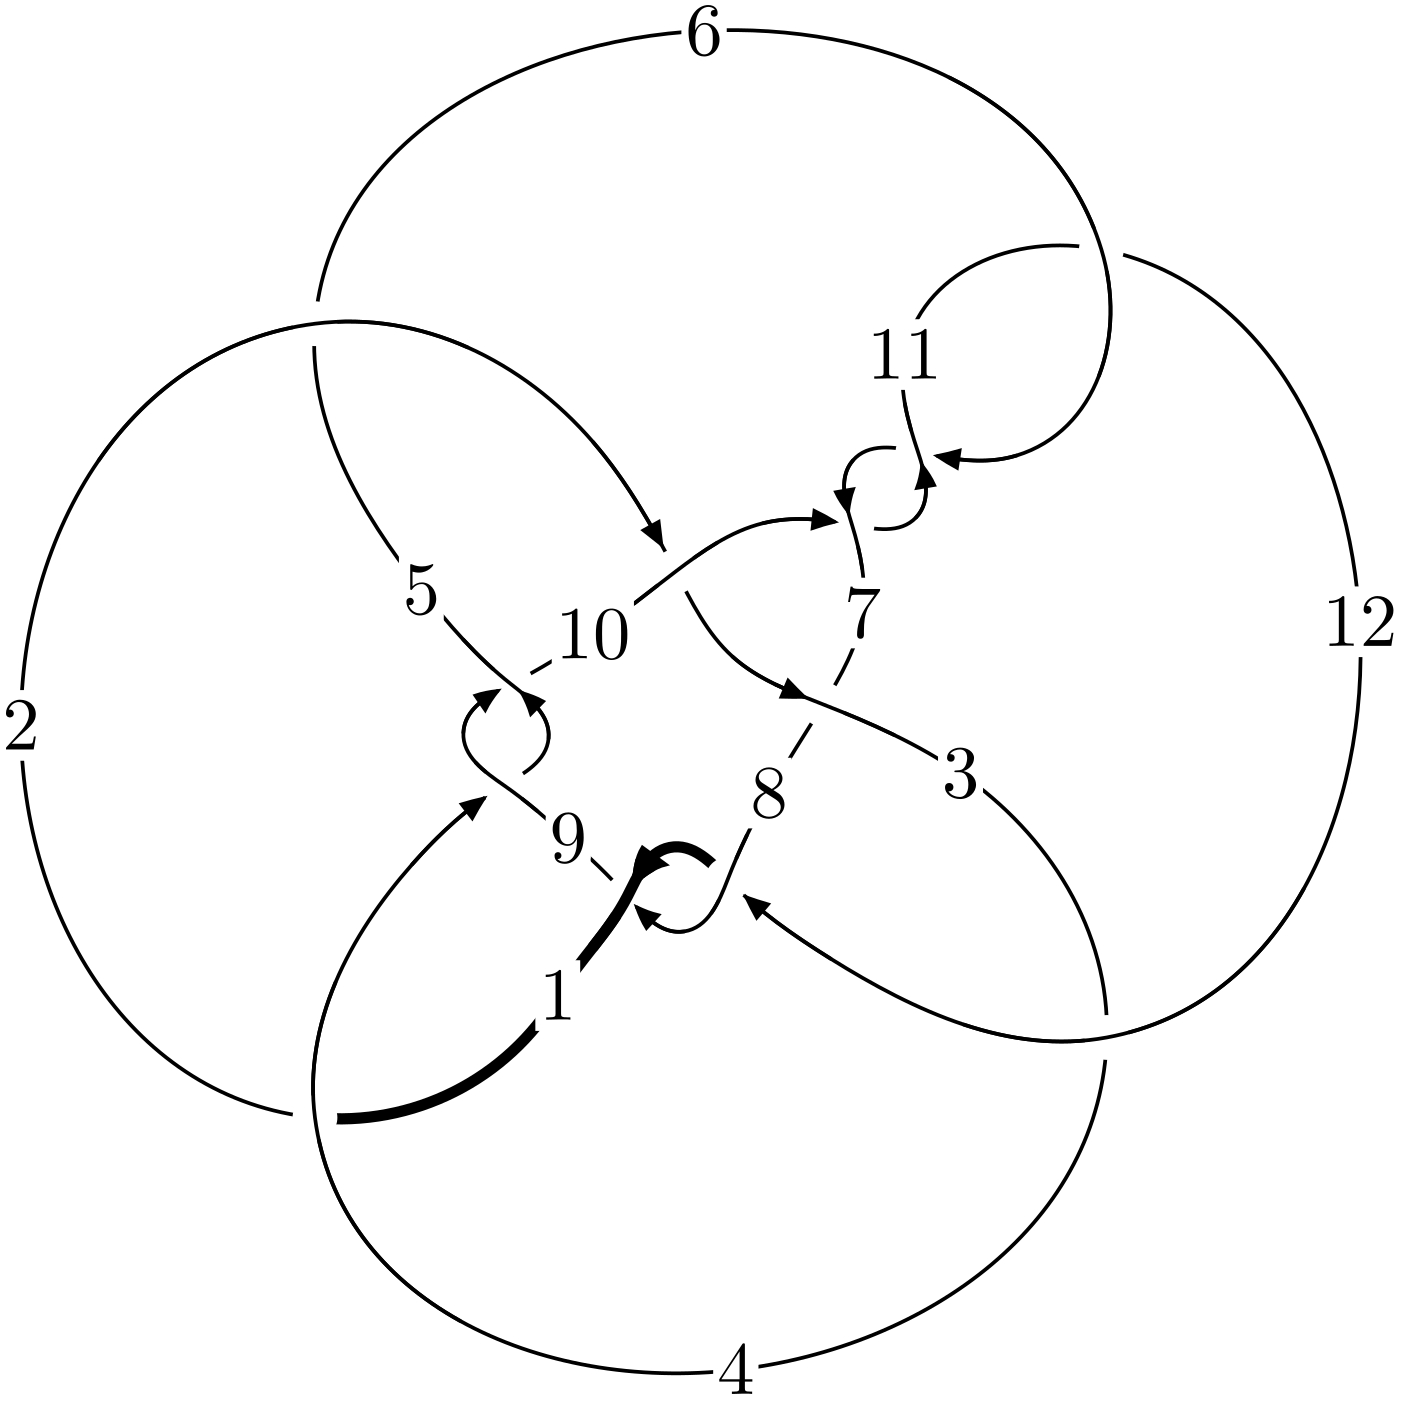
\includegraphics[width=112pt]{../../../GIT/diagram.site/Diagrams/png/2001_12a_1200.png}\\
\ \ \ A knot diagram\footnotemark}&
\allowdisplaybreaks
\textbf{Linearized knot diagam} \\
\cline{2-2}
 &
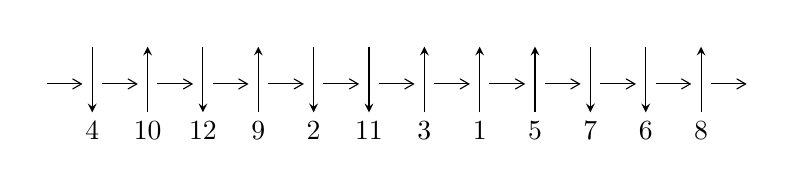
\begin{tikzpicture}[x=20pt, y=17pt]
	% nodes
	\node (C0) at (0, 0) {};
	\node (C1) at (1, 0) {};
	\node (C1U) at (1, +1) {};
	\node (C1D) at (1, -1) {4};

	\node (C2) at (2, 0) {};
	\node (C2U) at (2, +1) {};
	\node (C2D) at (2, -1) {10};

	\node (C3) at (3, 0) {};
	\node (C3U) at (3, +1) {};
	\node (C3D) at (3, -1) {12};

	\node (C4) at (4, 0) {};
	\node (C4U) at (4, +1) {};
	\node (C4D) at (4, -1) {9};

	\node (C5) at (5, 0) {};
	\node (C5U) at (5, +1) {};
	\node (C5D) at (5, -1) {2};

	\node (C6) at (6, 0) {};
	\node (C6U) at (6, +1) {};
	\node (C6D) at (6, -1) {11};

	\node (C7) at (7, 0) {};
	\node (C7U) at (7, +1) {};
	\node (C7D) at (7, -1) {3};

	\node (C8) at (8, 0) {};
	\node (C8U) at (8, +1) {};
	\node (C8D) at (8, -1) {1};

	\node (C9) at (9, 0) {};
	\node (C9U) at (9, +1) {};
	\node (C9D) at (9, -1) {5};

	\node (C10) at (10, 0) {};
	\node (C10U) at (10, +1) {};
	\node (C10D) at (10, -1) {7};

	\node (C11) at (11, 0) {};
	\node (C11U) at (11, +1) {};
	\node (C11D) at (11, -1) {6};

	\node (C12) at (12, 0) {};
	\node (C12U) at (12, +1) {};
	\node (C12D) at (12, -1) {8};
	\node (C13) at (13, 0) {};

	% arrows
	\draw[->,>={angle 60}]
	(C0) edge (C1) (C1) edge (C2) (C2) edge (C3) (C3) edge (C4) (C4) edge (C5) (C5) edge (C6) (C6) edge (C7) (C7) edge (C8) (C8) edge (C9) (C9) edge (C10) (C10) edge (C11) (C11) edge (C12) (C12) edge (C13) ;	\draw[->,>=stealth]
	(C1U) edge (C1D) (C2D) edge (C2U) (C3U) edge (C3D) (C4D) edge (C4U) (C5U) edge (C5D) (C6U) edge (C6D) (C7D) edge (C7U) (C8D) edge (C8U) (C9D) edge (C9U) (C10U) edge (C10D) (C11U) edge (C11D) (C12D) edge (C12U) ;
	\end{tikzpicture} \\
\hhline{~~} \\& 
\textbf{Solving Sequence} \\ \cline{2-2} 
 &
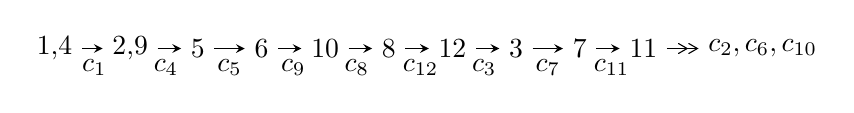
\begin{tikzpicture}[x=23pt, y=7pt]
	% node
	\node (A0) at (-1/8, 0) {1,4};
	\node (A1) at (17/16, 0) {2,9};
	\node (A2) at (17/8, 0) {5};
	\node (A3) at (25/8, 0) {6};
	\node (A4) at (33/8, 0) {10};
	\node (A5) at (41/8, 0) {8};
	\node (A6) at (49/8, 0) {12};
	\node (A7) at (57/8, 0) {3};
	\node (A8) at (65/8, 0) {7};
	\node (A9) at (73/8, 0) {11};
	\node (C1) at (1/2, -1) {$c_{1}$};
	\node (C2) at (13/8, -1) {$c_{4}$};
	\node (C3) at (21/8, -1) {$c_{5}$};
	\node (C4) at (29/8, -1) {$c_{9}$};
	\node (C5) at (37/8, -1) {$c_{8}$};
	\node (C6) at (45/8, -1) {$c_{12}$};
	\node (C7) at (53/8, -1) {$c_{3}$};
	\node (C8) at (61/8, -1) {$c_{7}$};
	\node (C9) at (69/8, -1) {$c_{11}$};
	\node (A10) at (11, 0) {$c_{2},c_{6},c_{10}$};

	% edge
	\draw[->,>=stealth]	
	(A0) edge (A1) (A1) edge (A2) (A2) edge (A3) (A3) edge (A4) (A4) edge (A5) (A5) edge (A6) (A6) edge (A7) (A7) edge (A8) (A8) edge (A9) ;
	\draw[->>,>={angle 60}]	
	(A9) edge (A10);
\end{tikzpicture} \\ 

\end{tabular} \\

\footnotetext{
The image of knot diagram is generated by the software ``\textbf{Draw programme}" developed by Andrew Bartholomew(\url{http://www.layer8.co.uk/maths/draw/index.htm\#Running-draw}), where we modified some parts for our purpose(\url{https://github.com/CATsTAILs/LinksPainter}).
}\phantom \\ \newline 
\centering \textbf{Ideals for irreducible components\footnotemark of $X_{\text{par}}$} 
 
\begin{align*}
I^u_{1}&=\langle 
-2.47770\times10^{71} u^{37}-6.71387\times10^{72} u^{36}+\cdots+8.89209\times10^{71} b+3.00786\times10^{74},\\
\phantom{I^u_{1}}&\phantom{= \langle  }-3.75982\times10^{73} u^{37}-1.01509\times10^{75} u^{36}+\cdots+1.35160\times10^{74} a+6.53327\times10^{76},\\
\phantom{I^u_{1}}&\phantom{= \langle  }u^{38}+28 u^{37}+\cdots-20672 u-1216\rangle \\
I^u_{2}&=\langle 
1.23963\times10^{66} u^{44}-1.60230\times10^{67} u^{43}+\cdots+2.01296\times10^{66} b-2.34540\times10^{67},\\
\phantom{I^u_{2}}&\phantom{= \langle  }2.22813\times10^{69} a u^{44}+2.15790\times10^{69} u^{44}+\cdots+2.36150\times10^{72} a-1.72905\times10^{72},\\
\phantom{I^u_{2}}&\phantom{= \langle  }u^{45}-14 u^{44}+\cdots+647 u-95\rangle \\
I^u_{3}&=\langle 
25355163523791 u^{16}-260299596465976 u^{15}+\cdots+37179633494568 b+433910338329094,\\
\phantom{I^u_{3}}&\phantom{= \langle  }433910338329094 u^{16}-4443396595810751 u^{15}+\cdots+483335235429384 a+6883326552789727,\\
\phantom{I^u_{3}}&\phantom{= \langle  }u^{17}-11 u^{16}+\cdots+61 u-13\rangle \\
I^u_{4}&=\langle 
u^6+u^3+a u+2 u^2+b,\;u^5 a-2 u^6+2 u^5- u^4+u^2 a-4 u^3+a^2+2 a u+2 u-4,\;u^7+2 u^4+2 u^3+u+1\rangle \\
\\
\end{align*}
\raggedright * 4 irreducible components of $\dim_{\mathbb{C}}=0$, with total 159 representations.\\
\footnotetext{All coefficients of polynomials are rational numbers. But the coefficients are sometimes approximated in decimal forms when there is not enough margin.}
\newpage
\renewcommand{\arraystretch}{1}
\centering \section*{I. $I^u_{1}= \langle -2.48\times10^{71} u^{37}-6.71\times10^{72} u^{36}+\cdots+8.89\times10^{71} b+3.01\times10^{74},\;-3.76\times10^{73} u^{37}-1.02\times10^{75} u^{36}+\cdots+1.35\times10^{74} a+6.53\times10^{76},\;u^{38}+28 u^{37}+\cdots-20672 u-1216 \rangle$}
\flushleft \textbf{(i) Arc colorings}\\
\begin{tabular}{m{7pt} m{180pt} m{7pt} m{180pt} }
\flushright $a_{1}=$&$\begin{pmatrix}1\\0\end{pmatrix}$ \\
\flushright $a_{4}=$&$\begin{pmatrix}0\\u\end{pmatrix}$ \\
\flushright $a_{2}=$&$\begin{pmatrix}1\\u^2\end{pmatrix}$ \\
\flushright $a_{9}=$&$\begin{pmatrix}0.278176 u^{37}+7.51030 u^{36}+\cdots-7216.69 u-483.374\\0.278641 u^{37}+7.55038 u^{36}+\cdots-5267.09 u-338.262\end{pmatrix}$ \\
\flushright $a_{5}=$&$\begin{pmatrix}0.424357 u^{37}+11.7318 u^{36}+\cdots-10457.3 u-615.084\\0.150150 u^{37}+4.27796 u^{36}+\cdots-8156.22 u-516.018\end{pmatrix}$ \\
\flushright $a_{6}=$&$\begin{pmatrix}0.200449 u^{37}+5.56029 u^{36}+\cdots-4888.93 u-281.649\\0.156639 u^{37}+4.39770 u^{36}+\cdots-6405.46 u-397.016\end{pmatrix}$ \\
\flushright $a_{10}=$&$\begin{pmatrix}1.33444 u^{37}+36.6406 u^{36}+\cdots-35526.8 u-2221.43\\0.472053 u^{37}+13.1388 u^{36}+\cdots-19942.2 u-1283.85\end{pmatrix}$ \\
\flushright $a_{8}=$&$\begin{pmatrix}-0.000464714 u^{37}-0.0400856 u^{36}+\cdots-1949.60 u-145.111\\0.278641 u^{37}+7.55038 u^{36}+\cdots-5267.09 u-338.262\end{pmatrix}$ \\
\flushright $a_{12}=$&$\begin{pmatrix}-0.274206 u^{37}-7.45387 u^{36}+\cdots+2300.05 u+100.066\\-0.150150 u^{37}-4.27796 u^{36}+\cdots+8157.22 u+516.018\end{pmatrix}$ \\
\flushright $a_{3}=$&$\begin{pmatrix}0.623672 u^{37}+17.0040 u^{36}+\cdots-7186.67 u-372.024\\0.332004 u^{37}+9.32506 u^{36}+\cdots-14197.7 u-889.830\end{pmatrix}$ \\
\flushright $a_{7}=$&$\begin{pmatrix}0.936820 u^{37}+25.3070 u^{36}+\cdots-10048.7 u-559.487\\0.968072 u^{37}+26.7304 u^{36}+\cdots-27389.6 u-1696.11\end{pmatrix}$ \\
\flushright $a_{11}=$&$\begin{pmatrix}-0.0194774 u^{37}-0.714546 u^{36}+\cdots+2524.43 u+121.508\\0.496891 u^{37}+13.3900 u^{36}+\cdots-1264.32 u-16.4375\end{pmatrix}$\\&\end{tabular}
\flushleft \textbf{(ii) Obstruction class $= -1$}\\~\\
\flushleft \textbf{(iii) Cusp Shapes $= 0.0832928 u^{37}+1.12467 u^{36}+\cdots+28762.4 u+1917.32$}\\~\\
\newpage\renewcommand{\arraystretch}{1}
\flushleft \textbf{(iv) u-Polynomials at the component}\newline \\
\begin{tabular}{m{50pt}|m{274pt}}
Crossings & \hspace{64pt}u-Polynomials at each crossing \\
\hline $$\begin{aligned}c_{1}\end{aligned}$$&$\begin{aligned}
&u^{38}-28 u^{37}+\cdots+20672 u-1216
\end{aligned}$\\
\hline $$\begin{aligned}c_{2},c_{7}\end{aligned}$$&$\begin{aligned}
&u^{38}+u^{37}+\cdots+3 u-1
\end{aligned}$\\
\hline $$\begin{aligned}c_{3},c_{5}\end{aligned}$$&$\begin{aligned}
&u^{38}-3 u^{37}+\cdots+54 u-7
\end{aligned}$\\
\hline $$\begin{aligned}c_{4},c_{8},c_{9}\\c_{12}\end{aligned}$$&$\begin{aligned}
&u^{38}-19 u^{36}+\cdots- u+1
\end{aligned}$\\
\hline $$\begin{aligned}c_{6},c_{10},c_{11}\end{aligned}$$&$\begin{aligned}
&u^{38}+8 u^{37}+\cdots-50 u-4
\end{aligned}$\\
\hline
\end{tabular}\\~\\
\newpage\renewcommand{\arraystretch}{1}
\flushleft \textbf{(v) Riley Polynomials at the component}\newline \\
\begin{tabular}{m{50pt}|m{274pt}}
Crossings & \hspace{64pt}Riley Polynomials at each crossing \\
\hline $$\begin{aligned}c_{1}\end{aligned}$$&$\begin{aligned}
&y^{38}-4 y^{37}+\cdots+24750464 y+1478656
\end{aligned}$\\
\hline $$\begin{aligned}c_{2},c_{7}\end{aligned}$$&$\begin{aligned}
&y^{38}-37 y^{37}+\cdots-51 y+1
\end{aligned}$\\
\hline $$\begin{aligned}c_{3},c_{5}\end{aligned}$$&$\begin{aligned}
&y^{38}+7 y^{37}+\cdots+948 y+49
\end{aligned}$\\
\hline $$\begin{aligned}c_{4},c_{8},c_{9}\\c_{12}\end{aligned}$$&$\begin{aligned}
&y^{38}-38 y^{37}+\cdots-35 y+1
\end{aligned}$\\
\hline $$\begin{aligned}c_{6},c_{10},c_{11}\end{aligned}$$&$\begin{aligned}
&y^{38}+36 y^{37}+\cdots-316 y+16
\end{aligned}$\\
\hline
\end{tabular}\\~\\
\newpage\flushleft \textbf{(vi) Complex Volumes and Cusp Shapes}
$$\begin{array}{c|c|c}  
\text{Solutions to }I^u_{1}& \I (\text{vol} + \sqrt{-1}CS) & \text{Cusp shape}\\
 \hline 
\begin{aligned}
u &= -0.682195 + 0.762723 I \\
a &= -0.498556 - 1.296080 I \\
b &= -1.32867 - 0.50392 I\end{aligned}
 & \phantom{-}5.16261 + 6.22750 I & \phantom{-0.000000 } 0 \\ \hline\begin{aligned}
u &= -0.682195 - 0.762723 I \\
a &= -0.498556 + 1.296080 I \\
b &= -1.32867 + 0.50392 I\end{aligned}
 & \phantom{-}5.16261 - 6.22750 I & \phantom{-0.000000 } 0 \\ \hline\begin{aligned}
u &= -0.948277 + 0.506166 I \\
a &= \phantom{-}0.357357 - 0.741251 I \\
b &= -0.036323 - 0.883794 I\end{aligned}
 & \phantom{-}4.64617 + 7.95698 I & \phantom{-0.000000 } 0 \\ \hline\begin{aligned}
u &= -0.948277 - 0.506166 I \\
a &= \phantom{-}0.357357 + 0.741251 I \\
b &= -0.036323 + 0.883794 I\end{aligned}
 & \phantom{-}4.64617 - 7.95698 I & \phantom{-0.000000 } 0 \\ \hline\begin{aligned}
u &= -0.294503 + 0.866980 I \\
a &= -0.585565 + 0.337901 I \\
b &= \phantom{-}0.120503 + 0.607186 I\end{aligned}
 & \phantom{-}6.70670 - 3.19363 I & \phantom{-0.000000 } 0 \\ \hline\begin{aligned}
u &= -0.294503 - 0.866980 I \\
a &= -0.585565 - 0.337901 I \\
b &= \phantom{-}0.120503 - 0.607186 I\end{aligned}
 & \phantom{-}6.70670 + 3.19363 I & \phantom{-0.000000 } 0 \\ \hline\begin{aligned}
u &= -0.809538 + 0.384223 I \\
a &= -0.450170 + 0.858186 I \\
b &= -0.034695 + 0.867701 I\end{aligned}
 & -1.50443 + 3.87717 I & \phantom{-0.000000 } 0. - 6.90669 I \\ \hline\begin{aligned}
u &= -0.809538 - 0.384223 I \\
a &= -0.450170 - 0.858186 I \\
b &= -0.034695 - 0.867701 I\end{aligned}
 & -1.50443 - 3.87717 I & \phantom{-0.000000 -}0. + 6.90669 I \\ \hline\begin{aligned}
u &= -0.078087 + 1.138990 I \\
a &= \phantom{-}0.084984 - 0.995053 I \\
b &= -1.126720 - 0.174497 I\end{aligned}
 & \phantom{-}7.14423 - 1.93403 I & \phantom{-0.000000 } 0 \\ \hline\begin{aligned}
u &= -0.078087 - 1.138990 I \\
a &= \phantom{-}0.084984 + 0.995053 I \\
b &= -1.126720 + 0.174497 I\end{aligned}
 & \phantom{-}7.14423 + 1.93403 I & \phantom{-0.000000 } 0\\
 \hline 
 \end{array}$$\newpage$$\begin{array}{c|c|c}  
\text{Solutions to }I^u_{1}& \I (\text{vol} + \sqrt{-1}CS) & \text{Cusp shape}\\
 \hline 
\begin{aligned}
u &= -1.19263\phantom{ +0.000000I} \\
a &= -1.16981\phantom{ +0.000000I} \\
b &= -1.39515\phantom{ +0.000000I}\end{aligned}
 & \phantom{-}8.14584\phantom{ +0.000000I} & \phantom{-0.000000 } 0 \\ \hline\begin{aligned}
u &= \phantom{-}1.19671\phantom{ +0.000000I} \\
a &= \phantom{-}0.140227\phantom{ +0.000000I} \\
b &= -0.167811\phantom{ +0.000000I}\end{aligned}
 & -2.28978\phantom{ +0.000000I} & \phantom{-0.000000 } 0 \\ \hline\begin{aligned}
u &= -0.409471 + 0.689495 I \\
a &= \phantom{-}0.28064 + 1.47948 I \\
b &= \phantom{-}1.135010 + 0.412302 I\end{aligned}
 & \phantom{-}2.51458 + 1.40446 I & \phantom{-0.000000 -}0. + 1.66220 I \\ \hline\begin{aligned}
u &= -0.409471 - 0.689495 I \\
a &= \phantom{-}0.28064 - 1.47948 I \\
b &= \phantom{-}1.135010 - 0.412302 I\end{aligned}
 & \phantom{-}2.51458 - 1.40446 I & \phantom{-0.000000 } 0. - 1.66220 I \\ \hline\begin{aligned}
u &= -0.486590 + 0.508142 I \\
a &= \phantom{-}1.33553 + 1.63331 I \\
b &= \phantom{-}1.47981 + 0.11611 I\end{aligned}
 & \phantom{-}13.69540 + 0.47437 I & \phantom{-}10.57797 + 0. I\phantom{ +0.000000I} \\ \hline\begin{aligned}
u &= -0.486590 - 0.508142 I \\
a &= \phantom{-}1.33553 - 1.63331 I \\
b &= \phantom{-}1.47981 - 0.11611 I\end{aligned}
 & \phantom{-}13.69540 - 0.47437 I & \phantom{-}10.57797 + 0. I\phantom{ +0.000000I} \\ \hline\begin{aligned}
u &= \phantom{-}1.254080 + 0.517048 I \\
a &= -0.211408 - 0.032930 I \\
b &= \phantom{-}0.248096 + 0.150605 I\end{aligned}
 & \phantom{-}1.85469 - 1.68737 I & \phantom{-0.000000 } 0 \\ \hline\begin{aligned}
u &= \phantom{-}1.254080 - 0.517048 I \\
a &= -0.211408 + 0.032930 I \\
b &= \phantom{-}0.248096 - 0.150605 I\end{aligned}
 & \phantom{-}1.85469 + 1.68737 I & \phantom{-0.000000 } 0 \\ \hline\begin{aligned}
u &= -0.534423 + 0.232538 I \\
a &= \phantom{-}0.849709 - 1.051240 I \\
b &= \phantom{-}0.209652 - 0.759395 I\end{aligned}
 & -0.216786 - 1.102140 I & \phantom{-}6.06046 - 0.98798 I \\ \hline\begin{aligned}
u &= -0.534423 - 0.232538 I \\
a &= \phantom{-}0.849709 + 1.051240 I \\
b &= \phantom{-}0.209652 + 0.759395 I\end{aligned}
 & -0.216786 + 1.102140 I & \phantom{-}6.06046 + 0.98798 I\\
 \hline 
 \end{array}$$\newpage$$\begin{array}{c|c|c}  
\text{Solutions to }I^u_{1}& \I (\text{vol} + \sqrt{-1}CS) & \text{Cusp shape}\\
 \hline 
\begin{aligned}
u &= -0.79600 + 1.25404 I \\
a &= \phantom{-}0.280283 + 1.010800 I \\
b &= \phantom{-}1.49069 + 0.45311 I\end{aligned}
 & \phantom{-}16.6042 + 5.5812 I & \phantom{-0.000000 } 0 \\ \hline\begin{aligned}
u &= -0.79600 - 1.25404 I \\
a &= \phantom{-}0.280283 - 1.010800 I \\
b &= \phantom{-}1.49069 - 0.45311 I\end{aligned}
 & \phantom{-}16.6042 - 5.5812 I & \phantom{-0.000000 } 0 \\ \hline\begin{aligned}
u &= -1.26064 + 1.00414 I \\
a &= -0.616800 - 0.532433 I \\
b &= -1.312200 - 0.051852 I\end{aligned}
 & \phantom{-}7.87194 - 0.16156 I & \phantom{-0.000000 } 0 \\ \hline\begin{aligned}
u &= -1.26064 - 1.00414 I \\
a &= -0.616800 + 0.532433 I \\
b &= -1.312200 + 0.051852 I\end{aligned}
 & \phantom{-}7.87194 + 0.16156 I & \phantom{-0.000000 } 0 \\ \hline\begin{aligned}
u &= -1.02376 + 1.27175 I \\
a &= -0.347514 - 0.890216 I \\
b &= -1.48790 - 0.46941 I\end{aligned}
 & \phantom{-}8.78158 + 8.86700 I & \phantom{-0.000000 } 0 \\ \hline\begin{aligned}
u &= -1.02376 - 1.27175 I \\
a &= -0.347514 + 0.890216 I \\
b &= -1.48790 + 0.46941 I\end{aligned}
 & \phantom{-}8.78158 - 8.86700 I & \phantom{-0.000000 } 0 \\ \hline\begin{aligned}
u &= -0.026194 + 0.314902 I \\
a &= \phantom{-}1.304250 + 0.123198 I \\
b &= \phantom{-}0.072959 - 0.407482 I\end{aligned}
 & \phantom{-}0.104937 - 1.022030 I & \phantom{-}1.88495 + 5.89504 I \\ \hline\begin{aligned}
u &= -0.026194 - 0.314902 I \\
a &= \phantom{-}1.304250 - 0.123198 I \\
b &= \phantom{-}0.072959 + 0.407482 I\end{aligned}
 & \phantom{-}0.104937 + 1.022030 I & \phantom{-}1.88495 - 5.89504 I \\ \hline\begin{aligned}
u &= -1.11118 + 1.40570 I \\
a &= \phantom{-}0.306522 + 0.814258 I \\
b &= \phantom{-}1.48520 + 0.47391 I\end{aligned}
 & \phantom{-}8.0623 + 14.2088 I & \phantom{-0.000000 } 0 \\ \hline\begin{aligned}
u &= -1.11118 - 1.40570 I \\
a &= \phantom{-}0.306522 - 0.814258 I \\
b &= \phantom{-}1.48520 - 0.47391 I\end{aligned}
 & \phantom{-}8.0623 - 14.2088 I & \phantom{-0.000000 } 0\\
 \hline 
 \end{array}$$\newpage$$\begin{array}{c|c|c}  
\text{Solutions to }I^u_{1}& \I (\text{vol} + \sqrt{-1}CS) & \text{Cusp shape}\\
 \hline 
\begin{aligned}
u &= -1.11056 + 1.52382 I \\
a &= -0.256748 - 0.786495 I \\
b &= -1.48361 - 0.48221 I\end{aligned}
 & \phantom{-}14.4591 + 18.3981 I & \phantom{-0.000000 } 0 \\ \hline\begin{aligned}
u &= -1.11056 - 1.52382 I \\
a &= -0.256748 + 0.786495 I \\
b &= -1.48361 + 0.48221 I\end{aligned}
 & \phantom{-}14.4591 - 18.3981 I & \phantom{-0.000000 } 0 \\ \hline\begin{aligned}
u &= -2.18875 + 0.58924 I \\
a &= \phantom{-}0.574000 + 0.132729 I \\
b &= \phantom{-}1.334550 - 0.047713 I\end{aligned}
 & \phantom{-}13.29000 + 2.22094 I & \phantom{-0.000000 } 0 \\ \hline\begin{aligned}
u &= -2.18875 - 0.58924 I \\
a &= \phantom{-}0.574000 - 0.132729 I \\
b &= \phantom{-}1.334550 + 0.047713 I\end{aligned}
 & \phantom{-}13.29000 - 2.22094 I & \phantom{-0.000000 } 0 \\ \hline\begin{aligned}
u &= -1.53894 + 1.77068 I \\
a &= \phantom{-}0.341740 + 0.404686 I \\
b &= \phantom{-}1.242490 + 0.017674 I\end{aligned}
 & \phantom{-}7.26991 - 3.65388 I & \phantom{-0.000000 } 0 \\ \hline\begin{aligned}
u &= -1.53894 - 1.77068 I \\
a &= \phantom{-}0.341740 - 0.404686 I \\
b &= \phantom{-}1.242490 - 0.017674 I\end{aligned}
 & \phantom{-}7.26991 + 3.65388 I & \phantom{-0.000000 } 0 \\ \hline\begin{aligned}
u &= -1.95702 + 2.08898 I \\
a &= -0.295957 - 0.310278 I \\
b &= -1.227360 + 0.011029 I\end{aligned}
 & \phantom{-}13.0421 - 6.7762 I & \phantom{-0.000000 } 0 \\ \hline\begin{aligned}
u &= -1.95702 - 2.08898 I \\
a &= -0.295957 + 0.310278 I \\
b &= -1.227360 - 0.011029 I\end{aligned}
 & \phantom{-}13.0421 + 6.7762 I & \phantom{-0.000000 } 0\\
 \hline 
 \end{array}$$\newpage\newpage\renewcommand{\arraystretch}{1}
\centering \section*{II. $I^u_{2}= \langle 1.24\times10^{66} u^{44}-1.60\times10^{67} u^{43}+\cdots+2.01\times10^{66} b-2.35\times10^{67},\;2.23\times10^{69} a u^{44}+2.16\times10^{69} u^{44}+\cdots+2.36\times10^{72} a-1.73\times10^{72},\;u^{45}-14 u^{44}+\cdots+647 u-95 \rangle$}
\flushleft \textbf{(i) Arc colorings}\\
\begin{tabular}{m{7pt} m{180pt} m{7pt} m{180pt} }
\flushright $a_{1}=$&$\begin{pmatrix}1\\0\end{pmatrix}$ \\
\flushright $a_{4}=$&$\begin{pmatrix}0\\u\end{pmatrix}$ \\
\flushright $a_{2}=$&$\begin{pmatrix}1\\u^2\end{pmatrix}$ \\
\flushright $a_{9}=$&$\begin{pmatrix}a\\-0.615824 u^{44}+7.95994 u^{43}+\cdots+50.6359 u+11.6515\end{pmatrix}$ \\
\flushright $a_{5}=$&$\begin{pmatrix}0.615824 a u^{44}-0.491264 u^{44}+\cdots-11.6515 a-11.2843\\-0.336732 u^{44}+4.56789 u^{43}+\cdots+307.564 u-46.6701\end{pmatrix}$ \\
\flushright $a_{6}=$&$\begin{pmatrix}0.929888 a u^{44}-0.300893 u^{44}+\cdots+51.1995 a+3.39628\\-0.382414 a u^{44}-0.271052 u^{44}+\cdots-10.1434 a-38.4007\end{pmatrix}$ \\
\flushright $a_{10}=$&$\begin{pmatrix}0.459564 a u^{44}+0.593910 u^{44}+\cdots+55.6239 a+93.8232\\0.146361 a u^{44}-0.615824 u^{44}+\cdots+31.9895 a+11.6515\end{pmatrix}$ \\
\flushright $a_{8}=$&$\begin{pmatrix}0.615824 u^{44}-7.95994 u^{43}+\cdots+a-11.6515\\-0.615824 u^{44}+7.95994 u^{43}+\cdots+50.6359 u+11.6515\end{pmatrix}$ \\
\flushright $a_{12}=$&$\begin{pmatrix}0.661589 a u^{44}-0.0317001 u^{44}+\cdots+58.5032 a+44.3396\\-0.661589 a u^{44}-0.459564 u^{44}+\cdots-58.5032 a-54.6239\end{pmatrix}$ \\
\flushright $a_{3}=$&$\begin{pmatrix}-0.0360838 a u^{44}+0.167204 u^{44}+\cdots+4.77789 a+46.2078\\0.103674 a u^{44}-0.311210 u^{44}+\cdots+31.7125 a-4.01151\end{pmatrix}$ \\
\flushright $a_{7}=$&$\begin{pmatrix}0.550513 a u^{44}-0.0645878 u^{44}+\cdots+35.7555 a+70.1492\\-0.0874292 a u^{44}-0.798455 u^{44}+\cdots+39.9458 a-99.3659\end{pmatrix}$ \\
\flushright $a_{11}=$&$\begin{pmatrix}0.680827 a u^{44}-0.423692 u^{44}+\cdots+153.624 a-54.8531\\-0.749233 a u^{44}+0.213638 u^{44}+\cdots-77.8171 a-54.6297\end{pmatrix}$\\&\end{tabular}
\flushleft \textbf{(ii) Obstruction class $= -1$}\\~\\
\flushleft \textbf{(iii) Cusp Shapes $= -3.08751 u^{44}+43.6285 u^{43}+\cdots+3503.19 u-546.068$}\\~\\
\newpage\renewcommand{\arraystretch}{1}
\flushleft \textbf{(iv) u-Polynomials at the component}\newline \\
\begin{tabular}{m{50pt}|m{274pt}}
Crossings & \hspace{64pt}u-Polynomials at each crossing \\
\hline $$\begin{aligned}c_{1}\end{aligned}$$&$\begin{aligned}
&(u^{45}+14 u^{44}+\cdots+647 u+95)^{2}
\end{aligned}$\\
\hline $$\begin{aligned}c_{2},c_{7}\end{aligned}$$&$\begin{aligned}
&u^{90}+2 u^{89}+\cdots+36484534 u+8946419
\end{aligned}$\\
\hline $$\begin{aligned}c_{3},c_{5}\end{aligned}$$&$\begin{aligned}
&u^{90}+3 u^{89}+\cdots-321472 u+57793
\end{aligned}$\\
\hline $$\begin{aligned}c_{4},c_{8},c_{9}\\c_{12}\end{aligned}$$&$\begin{aligned}
&u^{90}+u^{89}+\cdots-4 u^2+1
\end{aligned}$\\
\hline $$\begin{aligned}c_{6},c_{10},c_{11}\end{aligned}$$&$\begin{aligned}
&(u^{45}-3 u^{44}+\cdots+15 u^2-1)^{2}
\end{aligned}$\\
\hline
\end{tabular}\\~\\
\newpage\renewcommand{\arraystretch}{1}
\flushleft \textbf{(v) Riley Polynomials at the component}\newline \\
\begin{tabular}{m{50pt}|m{274pt}}
Crossings & \hspace{64pt}Riley Polynomials at each crossing \\
\hline $$\begin{aligned}c_{1}\end{aligned}$$&$\begin{aligned}
&(y^{45}+26 y^{44}+\cdots-136951 y-9025)^{2}
\end{aligned}$\\
\hline $$\begin{aligned}c_{2},c_{7}\end{aligned}$$&$\begin{aligned}
&y^{90}-20 y^{89}+\cdots-2040881454030634 y+80038412923561
\end{aligned}$\\
\hline $$\begin{aligned}c_{3},c_{5}\end{aligned}$$&$\begin{aligned}
&y^{90}+9 y^{89}+\cdots+26479752282 y+3340030849
\end{aligned}$\\
\hline $$\begin{aligned}c_{4},c_{8},c_{9}\\c_{12}\end{aligned}$$&$\begin{aligned}
&y^{90}-69 y^{89}+\cdots-8 y+1
\end{aligned}$\\
\hline $$\begin{aligned}c_{6},c_{10},c_{11}\end{aligned}$$&$\begin{aligned}
&(y^{45}+45 y^{44}+\cdots+30 y-1)^{2}
\end{aligned}$\\
\hline
\end{tabular}\\~\\
\newpage\flushleft \textbf{(vi) Complex Volumes and Cusp Shapes}
$$\begin{array}{c|c|c}  
\text{Solutions to }I^u_{2}& \I (\text{vol} + \sqrt{-1}CS) & \text{Cusp shape}\\
 \hline 
\begin{aligned}
u &= -0.611610 + 0.781700 I \\
a &= \phantom{-}0.729264 - 1.039030 I \\
b &= -1.262600 - 0.392766 I\end{aligned}
 & \phantom{-}2.32033 + 8.38253 I & \phantom{-0.000000 } 0. - 9.64974 I \\ \hline\begin{aligned}
u &= -0.611610 + 0.781700 I \\
a &= -0.472221 - 1.245730 I \\
b &= -0.366184 - 1.205550 I\end{aligned}
 & \phantom{-}2.32033 + 8.38253 I & \phantom{-0.000000 } 0. - 9.64974 I \\ \hline\begin{aligned}
u &= -0.611610 - 0.781700 I \\
a &= \phantom{-}0.729264 + 1.039030 I \\
b &= -1.262600 + 0.392766 I\end{aligned}
 & \phantom{-}2.32033 - 8.38253 I & \phantom{-0.000000 -}0. + 9.64974 I \\ \hline\begin{aligned}
u &= -0.611610 - 0.781700 I \\
a &= -0.472221 + 1.245730 I \\
b &= -0.366184 + 1.205550 I\end{aligned}
 & \phantom{-}2.32033 - 8.38253 I & \phantom{-0.000000 -}0. + 9.64974 I \\ \hline\begin{aligned}
u &= \phantom{-}0.539451 + 0.881956 I \\
a &= -0.829441 - 0.107208 I \\
b &= \phantom{-}1.250180 - 0.180411 I\end{aligned}
 & \phantom{-}1.59150 - 2.15051 I & \phantom{-0.000000 } 0 \\ \hline\begin{aligned}
u &= \phantom{-}0.539451 + 0.881956 I \\
a &= -0.482101 + 1.122630 I \\
b &= \phantom{-}0.352890 + 0.789364 I\end{aligned}
 & \phantom{-}1.59150 - 2.15051 I & \phantom{-0.000000 } 0 \\ \hline\begin{aligned}
u &= \phantom{-}0.539451 - 0.881956 I \\
a &= -0.829441 + 0.107208 I \\
b &= \phantom{-}1.250180 + 0.180411 I\end{aligned}
 & \phantom{-}1.59150 + 2.15051 I & \phantom{-0.000000 } 0 \\ \hline\begin{aligned}
u &= \phantom{-}0.539451 - 0.881956 I \\
a &= -0.482101 - 1.122630 I \\
b &= \phantom{-}0.352890 - 0.789364 I\end{aligned}
 & \phantom{-}1.59150 + 2.15051 I & \phantom{-0.000000 } 0 \\ \hline\begin{aligned}
u &= -0.149036 + 0.922013 I \\
a &= -0.001131 - 1.359660 I \\
b &= -0.247151 - 1.342480 I\end{aligned}
 & \phantom{-}10.83630 - 0.43960 I & \phantom{-}11.40794 + 0. I\phantom{ +0.000000I} \\ \hline\begin{aligned}
u &= -0.149036 + 0.922013 I \\
a &= \phantom{-}1.37673 - 0.49059 I \\
b &= -1.253790 - 0.201595 I\end{aligned}
 & \phantom{-}10.83630 - 0.43960 I & \phantom{-}11.40794 + 0. I\phantom{ +0.000000I}\\
 \hline 
 \end{array}$$\newpage$$\begin{array}{c|c|c}  
\text{Solutions to }I^u_{2}& \I (\text{vol} + \sqrt{-1}CS) & \text{Cusp shape}\\
 \hline 
\begin{aligned}
u &= -0.149036 - 0.922013 I \\
a &= -0.001131 + 1.359660 I \\
b &= -0.247151 + 1.342480 I\end{aligned}
 & \phantom{-}10.83630 + 0.43960 I & \phantom{-}11.40794 + 0. I\phantom{ +0.000000I} \\ \hline\begin{aligned}
u &= -0.149036 - 0.922013 I \\
a &= \phantom{-}1.37673 + 0.49059 I \\
b &= -1.253790 + 0.201595 I\end{aligned}
 & \phantom{-}10.83630 + 0.43960 I & \phantom{-}11.40794 + 0. I\phantom{ +0.000000I} \\ \hline\begin{aligned}
u &= \phantom{-}0.666316 + 0.841914 I \\
a &= \phantom{-}0.428169 - 0.840537 I \\
b &= \phantom{-}0.113870 - 0.741259 I\end{aligned}
 & -0.32693 - 2.59057 I & \phantom{-0.000000 } 0 \\ \hline\begin{aligned}
u &= \phantom{-}0.666316 + 0.841914 I \\
a &= \phantom{-}0.475542 + 0.511609 I \\
b &= -0.992955 + 0.199582 I\end{aligned}
 & -0.32693 - 2.59057 I & \phantom{-0.000000 } 0 \\ \hline\begin{aligned}
u &= \phantom{-}0.666316 - 0.841914 I \\
a &= \phantom{-}0.428169 + 0.840537 I \\
b &= \phantom{-}0.113870 + 0.741259 I\end{aligned}
 & -0.32693 + 2.59057 I & \phantom{-0.000000 } 0 \\ \hline\begin{aligned}
u &= \phantom{-}0.666316 - 0.841914 I \\
a &= \phantom{-}0.475542 - 0.511609 I \\
b &= -0.992955 - 0.199582 I\end{aligned}
 & -0.32693 + 2.59057 I & \phantom{-0.000000 } 0 \\ \hline\begin{aligned}
u &= \phantom{-}0.638115 + 0.635046 I \\
a &= \phantom{-}0.912716 + 0.034496 I \\
b &= -1.228450 + 0.253822 I\end{aligned}
 & \phantom{-}5.51564 - 1.64544 I & \phantom{-}5.84263 - 1.31809 I \\ \hline\begin{aligned}
u &= \phantom{-}0.638115 + 0.635046 I \\
a &= \phantom{-}0.768321 - 1.162400 I \\
b &= -0.560511 - 0.601629 I\end{aligned}
 & \phantom{-}5.51564 - 1.64544 I & \phantom{-}5.84263 - 1.31809 I \\ \hline\begin{aligned}
u &= \phantom{-}0.638115 - 0.635046 I \\
a &= \phantom{-}0.912716 - 0.034496 I \\
b &= -1.228450 - 0.253822 I\end{aligned}
 & \phantom{-}5.51564 + 1.64544 I & \phantom{-}5.84263 + 1.31809 I \\ \hline\begin{aligned}
u &= \phantom{-}0.638115 - 0.635046 I \\
a &= \phantom{-}0.768321 + 1.162400 I \\
b &= -0.560511 + 0.601629 I\end{aligned}
 & \phantom{-}5.51564 + 1.64544 I & \phantom{-}5.84263 + 1.31809 I\\
 \hline 
 \end{array}$$\newpage$$\begin{array}{c|c|c}  
\text{Solutions to }I^u_{2}& \I (\text{vol} + \sqrt{-1}CS) & \text{Cusp shape}\\
 \hline 
\begin{aligned}
u &= \phantom{-}1.11036\phantom{ +0.000000I} \\
a &= \phantom{-}0.144304 + 0.256392 I \\
b &= -0.160229 + 0.284686 I\end{aligned}
 & -2.27006\phantom{ +0.000000I} & \phantom{-0.000000 } 0 \\ \hline\begin{aligned}
u &= \phantom{-}1.11036\phantom{ +0.000000I} \\
a &= \phantom{-}0.144304 - 0.256392 I \\
b &= -0.160229 - 0.284686 I\end{aligned}
 & -2.27006\phantom{ +0.000000I} & \phantom{-0.000000 } 0 \\ \hline\begin{aligned}
u &= -0.775611 + 0.416273 I \\
a &= -1.56216 - 0.30077 I \\
b &= -0.121214 + 0.254236 I\end{aligned}
 & \phantom{-}8.62121 + 3.17668 I & \phantom{-}4.82175 - 5.04350 I \\ \hline\begin{aligned}
u &= -0.775611 + 0.416273 I \\
a &= -0.257914 + 0.189364 I \\
b &= -1.336830 + 0.417007 I\end{aligned}
 & \phantom{-}8.62121 + 3.17668 I & \phantom{-}4.82175 - 5.04350 I \\ \hline\begin{aligned}
u &= -0.775611 - 0.416273 I \\
a &= -1.56216 + 0.30077 I \\
b &= -0.121214 - 0.254236 I\end{aligned}
 & \phantom{-}8.62121 - 3.17668 I & \phantom{-}4.82175 + 5.04350 I \\ \hline\begin{aligned}
u &= -0.775611 - 0.416273 I \\
a &= -0.257914 - 0.189364 I \\
b &= -1.336830 - 0.417007 I\end{aligned}
 & \phantom{-}8.62121 - 3.17668 I & \phantom{-}4.82175 + 5.04350 I \\ \hline\begin{aligned}
u &= -0.681944 + 0.897038 I \\
a &= -0.690712 + 0.859416 I \\
b &= \phantom{-}1.309170 + 0.393232 I\end{aligned}
 & \phantom{-}8.8609 + 12.5151 I & \phantom{-0.000000 } 0 \\ \hline\begin{aligned}
u &= -0.681944 + 0.897038 I \\
a &= \phantom{-}0.425318 + 1.136100 I \\
b &= \phantom{-}0.299902 + 1.205670 I\end{aligned}
 & \phantom{-}8.8609 + 12.5151 I & \phantom{-0.000000 } 0 \\ \hline\begin{aligned}
u &= -0.681944 - 0.897038 I \\
a &= -0.690712 - 0.859416 I \\
b &= \phantom{-}1.309170 - 0.393232 I\end{aligned}
 & \phantom{-}8.8609 - 12.5151 I & \phantom{-0.000000 } 0 \\ \hline\begin{aligned}
u &= -0.681944 - 0.897038 I \\
a &= \phantom{-}0.425318 - 1.136100 I \\
b &= \phantom{-}0.299902 - 1.205670 I\end{aligned}
 & \phantom{-}8.8609 - 12.5151 I & \phantom{-0.000000 } 0\\
 \hline 
 \end{array}$$\newpage$$\begin{array}{c|c|c}  
\text{Solutions to }I^u_{2}& \I (\text{vol} + \sqrt{-1}CS) & \text{Cusp shape}\\
 \hline 
\begin{aligned}
u &= -0.211924 + 1.112060 I \\
a &= -0.479293 - 1.016480 I \\
b &= \phantom{-}0.066519 - 0.176869 I\end{aligned}
 & \phantom{-}3.71495 - 4.17242 I & \phantom{-0.000000 } 0 \\ \hline\begin{aligned}
u &= -0.211924 + 1.112060 I \\
a &= \phantom{-}0.164472 + 0.028472 I \\
b &= -1.231970 + 0.317586 I\end{aligned}
 & \phantom{-}3.71495 - 4.17242 I & \phantom{-0.000000 } 0 \\ \hline\begin{aligned}
u &= -0.211924 - 1.112060 I \\
a &= -0.479293 + 1.016480 I \\
b &= \phantom{-}0.066519 + 0.176869 I\end{aligned}
 & \phantom{-}3.71495 + 4.17242 I & \phantom{-0.000000 } 0 \\ \hline\begin{aligned}
u &= -0.211924 - 1.112060 I \\
a &= \phantom{-}0.164472 - 0.028472 I \\
b &= -1.231970 - 0.317586 I\end{aligned}
 & \phantom{-}3.71495 + 4.17242 I & \phantom{-0.000000 } 0 \\ \hline\begin{aligned}
u &= \phantom{-}0.653910 + 0.547063 I \\
a &= -1.086380 + 0.896906 I \\
b &= -1.91786 + 0.58852 I\end{aligned}
 & \phantom{-}5.97311 - 0.46804 I & \phantom{-}7.56258 + 9.30382 I \\ \hline\begin{aligned}
u &= \phantom{-}0.653910 + 0.547063 I \\
a &= \phantom{-}1.28241 - 1.97286 I \\
b &= \phantom{-}1.201060 + 0.007824 I\end{aligned}
 & \phantom{-}5.97311 - 0.46804 I & \phantom{-}7.56258 + 9.30382 I \\ \hline\begin{aligned}
u &= \phantom{-}0.653910 - 0.547063 I \\
a &= -1.086380 - 0.896906 I \\
b &= -1.91786 - 0.58852 I\end{aligned}
 & \phantom{-}5.97311 + 0.46804 I & \phantom{-}7.56258 - 9.30382 I \\ \hline\begin{aligned}
u &= \phantom{-}0.653910 - 0.547063 I \\
a &= \phantom{-}1.28241 + 1.97286 I \\
b &= \phantom{-}1.201060 - 0.007824 I\end{aligned}
 & \phantom{-}5.97311 + 0.46804 I & \phantom{-}7.56258 - 9.30382 I \\ \hline\begin{aligned}
u &= \phantom{-}0.576783 + 1.030760 I \\
a &= \phantom{-}0.873639 + 0.089311 I \\
b &= -1.318070 + 0.145393 I\end{aligned}
 & \phantom{-}6.72958 - 3.09750 I & \phantom{-0.000000 } 0 \\ \hline\begin{aligned}
u &= \phantom{-}0.576783 + 1.030760 I \\
a &= \phantom{-}0.437503 - 1.033930 I \\
b &= -0.411842 - 0.952021 I\end{aligned}
 & \phantom{-}6.72958 - 3.09750 I & \phantom{-0.000000 } 0\\
 \hline 
 \end{array}$$\newpage$$\begin{array}{c|c|c}  
\text{Solutions to }I^u_{2}& \I (\text{vol} + \sqrt{-1}CS) & \text{Cusp shape}\\
 \hline 
\begin{aligned}
u &= \phantom{-}0.576783 - 1.030760 I \\
a &= \phantom{-}0.873639 - 0.089311 I \\
b &= -1.318070 - 0.145393 I\end{aligned}
 & \phantom{-}6.72958 + 3.09750 I & \phantom{-0.000000 } 0 \\ \hline\begin{aligned}
u &= \phantom{-}0.576783 - 1.030760 I \\
a &= \phantom{-}0.437503 + 1.033930 I \\
b &= -0.411842 + 0.952021 I\end{aligned}
 & \phantom{-}6.72958 + 3.09750 I & \phantom{-0.000000 } 0 \\ \hline\begin{aligned}
u &= -0.418461 + 0.682095 I \\
a &= \phantom{-}0.41304 + 1.48489 I \\
b &= \phantom{-}0.452920 + 1.334230 I\end{aligned}
 & \phantom{-}2.86075 + 2.90624 I & \phantom{-}6.70323 - 8.96973 I \\ \hline\begin{aligned}
u &= -0.418461 + 0.682095 I \\
a &= -1.12521 + 1.35432 I \\
b &= \phantom{-}1.185680 + 0.339637 I\end{aligned}
 & \phantom{-}2.86075 + 2.90624 I & \phantom{-}6.70323 - 8.96973 I \\ \hline\begin{aligned}
u &= -0.418461 - 0.682095 I \\
a &= \phantom{-}0.41304 - 1.48489 I \\
b &= \phantom{-}0.452920 - 1.334230 I\end{aligned}
 & \phantom{-}2.86075 - 2.90624 I & \phantom{-}6.70323 + 8.96973 I \\ \hline\begin{aligned}
u &= -0.418461 - 0.682095 I \\
a &= -1.12521 - 1.35432 I \\
b &= \phantom{-}1.185680 - 0.339637 I\end{aligned}
 & \phantom{-}2.86075 - 2.90624 I & \phantom{-}6.70323 + 8.96973 I \\ \hline\begin{aligned}
u &= \phantom{-}1.178110 + 0.303143 I \\
a &= -0.326728 + 0.359344 I \\
b &= \phantom{-}0.011662 + 0.553716 I\end{aligned}
 & \phantom{-}1.78035 - 1.52529 I & \phantom{-0.000000 } 0 \\ \hline\begin{aligned}
u &= \phantom{-}1.178110 + 0.303143 I \\
a &= -0.122713 - 0.438429 I \\
b &= \phantom{-}0.493854 - 0.324300 I\end{aligned}
 & \phantom{-}1.78035 - 1.52529 I & \phantom{-0.000000 } 0 \\ \hline\begin{aligned}
u &= \phantom{-}1.178110 - 0.303143 I \\
a &= -0.326728 - 0.359344 I \\
b &= \phantom{-}0.011662 - 0.553716 I\end{aligned}
 & \phantom{-}1.78035 + 1.52529 I & \phantom{-0.000000 } 0 \\ \hline\begin{aligned}
u &= \phantom{-}1.178110 - 0.303143 I \\
a &= -0.122713 + 0.438429 I \\
b &= \phantom{-}0.493854 + 0.324300 I\end{aligned}
 & \phantom{-}1.78035 + 1.52529 I & \phantom{-0.000000 } 0\\
 \hline 
 \end{array}$$\newpage$$\begin{array}{c|c|c}  
\text{Solutions to }I^u_{2}& \I (\text{vol} + \sqrt{-1}CS) & \text{Cusp shape}\\
 \hline 
\begin{aligned}
u &= \phantom{-}0.354893 + 0.613023 I \\
a &= -0.80218 + 1.22978 I \\
b &= -0.253625 + 1.040460 I\end{aligned}
 & \phantom{-}1.59061 + 0.21798 I & \phantom{-}2.72267 + 0.45000 I \\ \hline\begin{aligned}
u &= \phantom{-}0.354893 + 0.613023 I \\
a &= -1.09182 - 1.04581 I \\
b &= \phantom{-}1.038570 + 0.055317 I\end{aligned}
 & \phantom{-}1.59061 + 0.21798 I & \phantom{-}2.72267 + 0.45000 I \\ \hline\begin{aligned}
u &= \phantom{-}0.354893 - 0.613023 I \\
a &= -0.80218 - 1.22978 I \\
b &= -0.253625 - 1.040460 I\end{aligned}
 & \phantom{-}1.59061 - 0.21798 I & \phantom{-}2.72267 - 0.45000 I \\ \hline\begin{aligned}
u &= \phantom{-}0.354893 - 0.613023 I \\
a &= -1.09182 + 1.04581 I \\
b &= \phantom{-}1.038570 - 0.055317 I\end{aligned}
 & \phantom{-}1.59061 - 0.21798 I & \phantom{-}2.72267 - 0.45000 I \\ \hline\begin{aligned}
u &= \phantom{-}0.712444 + 1.138040 I \\
a &= -0.212487 + 0.798192 I \\
b &= -0.154669 + 0.667898 I\end{aligned}
 & \phantom{-}4.38368 - 4.83757 I & \phantom{-0.000000 } 0 \\ \hline\begin{aligned}
u &= \phantom{-}0.712444 + 1.138040 I \\
a &= -0.360514 - 0.361601 I \\
b &= \phantom{-}1.059760 - 0.326849 I\end{aligned}
 & \phantom{-}4.38368 - 4.83757 I & \phantom{-0.000000 } 0 \\ \hline\begin{aligned}
u &= \phantom{-}0.712444 - 1.138040 I \\
a &= -0.212487 - 0.798192 I \\
b &= -0.154669 - 0.667898 I\end{aligned}
 & \phantom{-}4.38368 + 4.83757 I & \phantom{-0.000000 } 0 \\ \hline\begin{aligned}
u &= \phantom{-}0.712444 - 1.138040 I \\
a &= -0.360514 + 0.361601 I \\
b &= \phantom{-}1.059760 + 0.326849 I\end{aligned}
 & \phantom{-}4.38368 + 4.83757 I & \phantom{-0.000000 } 0 \\ \hline\begin{aligned}
u &= \phantom{-}0.793086 + 1.112180 I \\
a &= \phantom{-}0.482589 - 0.784671 I \\
b &= \phantom{-}1.56067 - 0.52472 I\end{aligned}
 & \phantom{-}7.73394 - 5.25113 I & \phantom{-0.000000 } 0 \\ \hline\begin{aligned}
u &= \phantom{-}0.793086 + 1.112180 I \\
a &= -0.350583 + 1.153260 I \\
b &= -1.255430 + 0.085588 I\end{aligned}
 & \phantom{-}7.73394 - 5.25113 I & \phantom{-0.000000 } 0\\
 \hline 
 \end{array}$$\newpage$$\begin{array}{c|c|c}  
\text{Solutions to }I^u_{2}& \I (\text{vol} + \sqrt{-1}CS) & \text{Cusp shape}\\
 \hline 
\begin{aligned}
u &= \phantom{-}0.793086 - 1.112180 I \\
a &= \phantom{-}0.482589 + 0.784671 I \\
b &= \phantom{-}1.56067 + 0.52472 I\end{aligned}
 & \phantom{-}7.73394 + 5.25113 I & \phantom{-0.000000 } 0 \\ \hline\begin{aligned}
u &= \phantom{-}0.793086 - 1.112180 I \\
a &= -0.350583 - 1.153260 I \\
b &= -1.255430 - 0.085588 I\end{aligned}
 & \phantom{-}7.73394 + 5.25113 I & \phantom{-0.000000 } 0 \\ \hline\begin{aligned}
u &= \phantom{-}0.253150 + 0.576313 I \\
a &= \phantom{-}0.93483 - 1.72737 I \\
b &= \phantom{-}1.69263 - 0.97809 I\end{aligned}
 & \phantom{-}12.01940 + 4.51852 I & \phantom{-}17.3811 - 5.6393 I \\ \hline\begin{aligned}
u &= \phantom{-}0.253150 + 0.576313 I \\
a &= \phantom{-}0.34122 + 3.08688 I \\
b &= -1.232160 - 0.101472 I\end{aligned}
 & \phantom{-}12.01940 + 4.51852 I & \phantom{-}17.3811 - 5.6393 I \\ \hline\begin{aligned}
u &= \phantom{-}0.253150 - 0.576313 I \\
a &= \phantom{-}0.93483 + 1.72737 I \\
b &= \phantom{-}1.69263 + 0.97809 I\end{aligned}
 & \phantom{-}12.01940 - 4.51852 I & \phantom{-}17.3811 + 5.6393 I \\ \hline\begin{aligned}
u &= \phantom{-}0.253150 - 0.576313 I \\
a &= \phantom{-}0.34122 - 3.08688 I \\
b &= -1.232160 + 0.101472 I\end{aligned}
 & \phantom{-}12.01940 - 4.51852 I & \phantom{-}17.3811 + 5.6393 I \\ \hline\begin{aligned}
u &= \phantom{-}0.486761 + 1.290350 I \\
a &= -0.288375 + 0.934430 I \\
b &= -1.48316 + 0.65192 I\end{aligned}
 & \phantom{-}15.0045 - 7.7049 I & \phantom{-0.000000 } 0 \\ \hline\begin{aligned}
u &= \phantom{-}0.486761 + 1.290350 I \\
a &= -0.062701 - 1.173080 I \\
b &= \phantom{-}1.346110 - 0.082739 I\end{aligned}
 & \phantom{-}15.0045 - 7.7049 I & \phantom{-0.000000 } 0 \\ \hline\begin{aligned}
u &= \phantom{-}0.486761 - 1.290350 I \\
a &= -0.288375 - 0.934430 I \\
b &= -1.48316 - 0.65192 I\end{aligned}
 & \phantom{-}15.0045 + 7.7049 I & \phantom{-0.000000 } 0 \\ \hline\begin{aligned}
u &= \phantom{-}0.486761 - 1.290350 I \\
a &= -0.062701 + 1.173080 I \\
b &= \phantom{-}1.346110 + 0.082739 I\end{aligned}
 & \phantom{-}15.0045 + 7.7049 I & \phantom{-0.000000 } 0\\
 \hline 
 \end{array}$$\newpage$$\begin{array}{c|c|c}  
\text{Solutions to }I^u_{2}& \I (\text{vol} + \sqrt{-1}CS) & \text{Cusp shape}\\
 \hline 
\begin{aligned}
u &= -0.298408 + 0.518145 I \\
a &= \phantom{-}0.160912 + 0.325351 I \\
b &= \phantom{-}1.331610 - 0.284286 I\end{aligned}
 & \phantom{-}3.05397 - 0.51778 I & \phantom{-}4.68541 - 4.29429 I \\ \hline\begin{aligned}
u &= -0.298408 + 0.518145 I \\
a &= \phantom{-}1.52344 + 1.69258 I \\
b &= \phantom{-}0.216596 + 0.013712 I\end{aligned}
 & \phantom{-}3.05397 - 0.51778 I & \phantom{-}4.68541 - 4.29429 I \\ \hline\begin{aligned}
u &= -0.298408 - 0.518145 I \\
a &= \phantom{-}0.160912 - 0.325351 I \\
b &= \phantom{-}1.331610 + 0.284286 I\end{aligned}
 & \phantom{-}3.05397 + 0.51778 I & \phantom{-}4.68541 + 4.29429 I \\ \hline\begin{aligned}
u &= -0.298408 - 0.518145 I \\
a &= \phantom{-}1.52344 - 1.69258 I \\
b &= \phantom{-}0.216596 - 0.013712 I\end{aligned}
 & \phantom{-}3.05397 + 0.51778 I & \phantom{-}4.68541 + 4.29429 I \\ \hline\begin{aligned}
u &= -0.48885 + 1.42397 I \\
a &= \phantom{-}0.480075 + 0.691881 I \\
b &= -0.228923 + 0.089425 I\end{aligned}
 & \phantom{-}9.94023 - 6.86720 I & \phantom{-0.000000 } 0 \\ \hline\begin{aligned}
u &= -0.48885 + 1.42397 I \\
a &= -0.105551 - 0.124529 I \\
b &= \phantom{-}1.219900 - 0.345387 I\end{aligned}
 & \phantom{-}9.94023 - 6.86720 I & \phantom{-0.000000 } 0 \\ \hline\begin{aligned}
u &= -0.48885 - 1.42397 I \\
a &= \phantom{-}0.480075 - 0.691881 I \\
b &= -0.228923 - 0.089425 I\end{aligned}
 & \phantom{-}9.94023 + 6.86720 I & \phantom{-0.000000 } 0 \\ \hline\begin{aligned}
u &= -0.48885 - 1.42397 I \\
a &= -0.105551 + 0.124529 I \\
b &= \phantom{-}1.219900 + 0.345387 I\end{aligned}
 & \phantom{-}9.94023 + 6.86720 I & \phantom{-0.000000 } 0 \\ \hline\begin{aligned}
u &= \phantom{-}1.30403 + 1.57384 I \\
a &= -0.317525 + 0.634119 I \\
b &= -1.138430 + 0.205272 I\end{aligned}
 & \phantom{-}7.21426 - 4.49667 I & \phantom{-0.000000 } 0 \\ \hline\begin{aligned}
u &= \phantom{-}1.30403 + 1.57384 I \\
a &= \phantom{-}0.278035 - 0.492975 I \\
b &= \phantom{-}1.41206 - 0.32718 I\end{aligned}
 & \phantom{-}7.21426 - 4.49667 I & \phantom{-0.000000 } 0\\
 \hline 
 \end{array}$$\newpage$$\begin{array}{c|c|c}  
\text{Solutions to }I^u_{2}& \I (\text{vol} + \sqrt{-1}CS) & \text{Cusp shape}\\
 \hline 
\begin{aligned}
u &= \phantom{-}1.30403 - 1.57384 I \\
a &= -0.317525 - 0.634119 I \\
b &= -1.138430 - 0.205272 I\end{aligned}
 & \phantom{-}7.21426 + 4.49667 I & \phantom{-0.000000 } 0 \\ \hline\begin{aligned}
u &= \phantom{-}1.30403 - 1.57384 I \\
a &= \phantom{-}0.278035 + 0.492975 I \\
b &= \phantom{-}1.41206 + 0.32718 I\end{aligned}
 & \phantom{-}7.21426 + 4.49667 I & \phantom{-0.000000 } 0 \\ \hline\begin{aligned}
u &= \phantom{-}1.03866 + 1.81167 I \\
a &= \phantom{-}0.185228 - 0.628944 I \\
b &= \phantom{-}1.165440 - 0.361396 I\end{aligned}
 & \phantom{-}4.20549 - 6.43436 I & \phantom{-0.000000 } 0 \\ \hline\begin{aligned}
u &= \phantom{-}1.03866 + 1.81167 I \\
a &= -0.127441 + 0.570229 I \\
b &= -1.331830 + 0.317689 I\end{aligned}
 & \phantom{-}4.20549 - 6.43436 I & \phantom{-0.000000 } 0 \\ \hline\begin{aligned}
u &= \phantom{-}1.03866 - 1.81167 I \\
a &= \phantom{-}0.185228 + 0.628944 I \\
b &= \phantom{-}1.165440 + 0.361396 I\end{aligned}
 & \phantom{-}4.20549 + 6.43436 I & \phantom{-0.000000 } 0 \\ \hline\begin{aligned}
u &= \phantom{-}1.03866 - 1.81167 I \\
a &= -0.127441 - 0.570229 I \\
b &= -1.331830 - 0.317689 I\end{aligned}
 & \phantom{-}4.20549 + 6.43436 I & \phantom{-0.000000 } 0 \\ \hline\begin{aligned}
u &= \phantom{-}0.88495 + 1.89707 I \\
a &= -0.144548 + 0.642165 I \\
b &= -1.139300 + 0.488014 I\end{aligned}
 & \phantom{-}9.10603 - 8.38435 I & \phantom{-0.000000 } 0 \\ \hline\begin{aligned}
u &= \phantom{-}0.88495 + 1.89707 I \\
a &= \phantom{-}0.018811 - 0.591785 I \\
b &= \phantom{-}1.346150 - 0.294066 I\end{aligned}
 & \phantom{-}9.10603 - 8.38435 I & \phantom{-0.000000 } 0 \\ \hline\begin{aligned}
u &= \phantom{-}0.88495 - 1.89707 I \\
a &= -0.144548 - 0.642165 I \\
b &= -1.139300 - 0.488014 I\end{aligned}
 & \phantom{-}9.10603 + 8.38435 I & \phantom{-0.000000 } 0 \\ \hline\begin{aligned}
u &= \phantom{-}0.88495 - 1.89707 I \\
a &= \phantom{-}0.018811 + 0.591785 I \\
b &= \phantom{-}1.346150 + 0.294066 I\end{aligned}
 & \phantom{-}9.10603 + 8.38435 I & \phantom{-0.000000 } 0\\
 \hline 
 \end{array}$$\newpage\newpage\renewcommand{\arraystretch}{1}
\centering \section*{III. $I^u_{3}= \langle 2.54\times10^{13} u^{16}-2.60\times10^{14} u^{15}+\cdots+3.72\times10^{13} b+4.34\times10^{14},\;4.34\times10^{14} u^{16}-4.44\times10^{15} u^{15}+\cdots+4.83\times10^{14} a+6.88\times10^{15},\;u^{17}-11 u^{16}+\cdots+61 u-13 \rangle$}
\flushleft \textbf{(i) Arc colorings}\\
\begin{tabular}{m{7pt} m{180pt} m{7pt} m{180pt} }
\flushright $a_{1}=$&$\begin{pmatrix}1\\0\end{pmatrix}$ \\
\flushright $a_{4}=$&$\begin{pmatrix}0\\u\end{pmatrix}$ \\
\flushright $a_{2}=$&$\begin{pmatrix}1\\u^2\end{pmatrix}$ \\
\flushright $a_{9}=$&$\begin{pmatrix}-0.897742 u^{16}+9.19320 u^{15}+\cdots+51.7535 u-14.2413\\-0.681964 u^{16}+7.00113 u^{15}+\cdots+40.5210 u-11.6706\end{pmatrix}$ \\
\flushright $a_{5}=$&$\begin{pmatrix}-0.580585 u^{16}+5.92362 u^{15}+\cdots+27.9777 u-9.09389\\-0.462812 u^{16}+4.80350 u^{15}+\cdots+27.3218 u-7.54760\end{pmatrix}$ \\
\flushright $a_{6}=$&$\begin{pmatrix}-0.405201 u^{16}+4.13662 u^{15}+\cdots+21.3399 u-7.56285\\-0.375250 u^{16}+3.87515 u^{15}+\cdots+20.9267 u-5.69881\end{pmatrix}$ \\
\flushright $a_{10}=$&$\begin{pmatrix}-1.05032 u^{16}+10.7472 u^{15}+\cdots+64.2093 u-17.6504\\-0.305860 u^{16}+3.10669 u^{15}+\cdots+16.4902 u-4.78869\end{pmatrix}$ \\
\flushright $a_{8}=$&$\begin{pmatrix}-0.215778 u^{16}+2.19206 u^{15}+\cdots+11.2325 u-2.57066\\-0.681964 u^{16}+7.00113 u^{15}+\cdots+40.5210 u-11.6706\end{pmatrix}$ \\
\flushright $a_{12}=$&$\begin{pmatrix}-0.117773 u^{16}+1.12012 u^{15}+\cdots+1.65596 u-0.546296\\-0.462812 u^{16}+4.80350 u^{15}+\cdots+26.3218 u-7.54760\end{pmatrix}$ \\
\flushright $a_{3}=$&$\begin{pmatrix}-0.194696 u^{16}+1.96627 u^{15}+\cdots+15.1175 u-4.23860\\-0.175383 u^{16}+1.78700 u^{15}+\cdots+7.63785 u-2.53105\end{pmatrix}$ \\
\flushright $a_{7}=$&$\begin{pmatrix}-0.0383098 u^{16}+0.354981 u^{15}+\cdots-3.47878 u+1.37647\\-0.566894 u^{16}+5.77956 u^{15}+\cdots+33.6425 u-9.36356\end{pmatrix}$ \\
\flushright $a_{11}=$&$\begin{pmatrix}-1.28094 u^{16}+13.1157 u^{15}+\cdots+65.7878 u-20.0167\\-0.489126 u^{16}+5.04876 u^{15}+\cdots+30.3915 u-8.70823\end{pmatrix}$\\&\end{tabular}
\flushleft \textbf{(ii) Obstruction class $= 1$}\\~\\
\flushleft \textbf{(iii) Cusp Shapes $= \frac{14747391055457}{3098302791214} u^{16}-\frac{590594498534627}{12393211164856} u^{15}+\cdots-\frac{1018255900118941}{4647454186821} u+\frac{2397735479791261}{37179633494568}$}\\~\\
\newpage\renewcommand{\arraystretch}{1}
\flushleft \textbf{(iv) u-Polynomials at the component}\newline \\
\begin{tabular}{m{50pt}|m{274pt}}
Crossings & \hspace{64pt}u-Polynomials at each crossing \\
\hline $$\begin{aligned}c_{1}\end{aligned}$$&$\begin{aligned}
&u^{17}-11 u^{16}+\cdots+61 u-13
\end{aligned}$\\
\hline $$\begin{aligned}c_{2},c_{7}\end{aligned}$$&$\begin{aligned}
&u^{17}- u^{16}+\cdots+5 u^2+1
\end{aligned}$\\
\hline $$\begin{aligned}c_{3},c_{5}\end{aligned}$$&$\begin{aligned}
&u^{17}+3 u^{16}+\cdots+3 u+1
\end{aligned}$\\
\hline $$\begin{aligned}c_{4},c_{8}\end{aligned}$$&$\begin{aligned}
&u^{17}-7 u^{15}+\cdots-7 u^2+1
\end{aligned}$\\
\hline $$\begin{aligned}c_{6}\end{aligned}$$&$\begin{aligned}
&u^{17}+3 u^{16}+\cdots-2 u-1
\end{aligned}$\\
\hline $$\begin{aligned}c_{9},c_{12}\end{aligned}$$&$\begin{aligned}
&u^{17}-7 u^{15}+\cdots+7 u^2-1
\end{aligned}$\\
\hline $$\begin{aligned}c_{10},c_{11}\end{aligned}$$&$\begin{aligned}
&u^{17}-3 u^{16}+\cdots-2 u+1
\end{aligned}$\\
\hline
\end{tabular}\\~\\
\newpage\renewcommand{\arraystretch}{1}
\flushleft \textbf{(v) Riley Polynomials at the component}\newline \\
\begin{tabular}{m{50pt}|m{274pt}}
Crossings & \hspace{64pt}Riley Polynomials at each crossing \\
\hline $$\begin{aligned}c_{1}\end{aligned}$$&$\begin{aligned}
&y^{17}+13 y^{16}+\cdots-829 y-169
\end{aligned}$\\
\hline $$\begin{aligned}c_{2},c_{7}\end{aligned}$$&$\begin{aligned}
&y^{17}+3 y^{16}+\cdots-10 y-1
\end{aligned}$\\
\hline $$\begin{aligned}c_{3},c_{5}\end{aligned}$$&$\begin{aligned}
&y^{17}+3 y^{16}+\cdots-5 y-1
\end{aligned}$\\
\hline $$\begin{aligned}c_{4},c_{8},c_{9}\\c_{12}\end{aligned}$$&$\begin{aligned}
&y^{17}-14 y^{16}+\cdots+14 y-1
\end{aligned}$\\
\hline $$\begin{aligned}c_{6},c_{10},c_{11}\end{aligned}$$&$\begin{aligned}
&y^{17}+17 y^{16}+\cdots+18 y^2-1
\end{aligned}$\\
\hline
\end{tabular}\\~\\
\newpage\flushleft \textbf{(vi) Complex Volumes and Cusp Shapes}
$$\begin{array}{c|c|c}  
\text{Solutions to }I^u_{3}& \I (\text{vol} + \sqrt{-1}CS) & \text{Cusp shape}\\
 \hline 
\begin{aligned}
u &= \phantom{-}0.672523 + 0.994302 I \\
a &= -0.231992 + 1.105750 I \\
b &= -1.255470 + 0.512970 I\end{aligned}
 & \phantom{-}4.86856 - 6.83059 I & \phantom{-}4.20585 + 10.23104 I \\ \hline\begin{aligned}
u &= \phantom{-}0.672523 - 0.994302 I \\
a &= -0.231992 - 1.105750 I \\
b &= -1.255470 - 0.512970 I\end{aligned}
 & \phantom{-}4.86856 + 6.83059 I & \phantom{-}4.20585 - 10.23104 I \\ \hline\begin{aligned}
u &= \phantom{-}0.739575 + 0.064407 I \\
a &= \phantom{-}0.475693 + 0.886639 I \\
b &= \phantom{-}0.294705 + 0.686375 I\end{aligned}
 & -0.84670 + 1.37045 I & -5.30898 - 4.32463 I \\ \hline\begin{aligned}
u &= \phantom{-}0.739575 - 0.064407 I \\
a &= \phantom{-}0.475693 - 0.886639 I \\
b &= \phantom{-}0.294705 - 0.686375 I\end{aligned}
 & -0.84670 - 1.37045 I & -5.30898 + 4.32463 I \\ \hline\begin{aligned}
u &= \phantom{-}1.29126\phantom{ +0.000000I} \\
a &= \phantom{-}0.338230\phantom{ +0.000000I} \\
b &= \phantom{-}0.436742\phantom{ +0.000000I}\end{aligned}
 & -2.05037\phantom{ +0.000000I} & \phantom{-}18.8440\phantom{ +0.000000I} \\ \hline\begin{aligned}
u &= \phantom{-}0.227690 + 0.618552 I \\
a &= -0.24105 - 1.81338 I \\
b &= \phantom{-}1.066790 - 0.561990 I\end{aligned}
 & \phantom{-}3.26404 - 1.84385 I & \phantom{-}9.66761 + 2.94728 I \\ \hline\begin{aligned}
u &= \phantom{-}0.227690 - 0.618552 I \\
a &= -0.24105 + 1.81338 I \\
b &= \phantom{-}1.066790 + 0.561990 I\end{aligned}
 & \phantom{-}3.26404 + 1.84385 I & \phantom{-}9.66761 - 2.94728 I \\ \hline\begin{aligned}
u &= \phantom{-}1.39451 + 0.50448 I \\
a &= -0.386813 + 0.041871 I \\
b &= -0.560538 - 0.136750 I\end{aligned}
 & \phantom{-}2.28339 - 1.51196 I & \phantom{-}11.74266 - 3.04379 I \\ \hline\begin{aligned}
u &= \phantom{-}1.39451 - 0.50448 I \\
a &= -0.386813 - 0.041871 I \\
b &= -0.560538 + 0.136750 I\end{aligned}
 & \phantom{-}2.28339 + 1.51196 I & \phantom{-}11.74266 + 3.04379 I \\ \hline\begin{aligned}
u &= -0.221722 + 0.326447 I \\
a &= \phantom{-}2.34722 + 1.33971 I \\
b &= -0.957777 + 0.469199 I\end{aligned}
 & \phantom{-}9.57721 + 2.19585 I & \phantom{-}10.18532 - 0.67460 I\\
 \hline 
 \end{array}$$\newpage$$\begin{array}{c|c|c}  
\text{Solutions to }I^u_{3}& \I (\text{vol} + \sqrt{-1}CS) & \text{Cusp shape}\\
 \hline 
\begin{aligned}
u &= -0.221722 - 0.326447 I \\
a &= \phantom{-}2.34722 - 1.33971 I \\
b &= -0.957777 - 0.469199 I\end{aligned}
 & \phantom{-}9.57721 - 2.19585 I & \phantom{-}10.18532 + 0.67460 I \\ \hline\begin{aligned}
u &= \phantom{-}0.70704 + 1.73293 I \\
a &= -0.071556 + 0.682925 I \\
b &= -1.234060 + 0.358853 I\end{aligned}
 & \phantom{-}5.17054 - 6.41143 I & \phantom{-}8.12565 + 7.83272 I \\ \hline\begin{aligned}
u &= \phantom{-}0.70704 - 1.73293 I \\
a &= -0.071556 - 0.682925 I \\
b &= -1.234060 - 0.358853 I\end{aligned}
 & \phantom{-}5.17054 + 6.41143 I & \phantom{-}8.12565 - 7.83272 I \\ \hline\begin{aligned}
u &= -0.06721 + 1.99987 I \\
a &= -0.186400 - 0.566671 I \\
b &= \phantom{-}1.145800 - 0.334688 I\end{aligned}
 & \phantom{-}11.28100 - 8.47803 I & \phantom{-}10.04502 + 7.78423 I \\ \hline\begin{aligned}
u &= -0.06721 - 1.99987 I \\
a &= -0.186400 + 0.566671 I \\
b &= \phantom{-}1.145800 + 0.334688 I\end{aligned}
 & \phantom{-}11.28100 + 8.47803 I & \phantom{-}10.04502 - 7.78423 I \\ \hline\begin{aligned}
u &= \phantom{-}1.40196 + 2.02720 I \\
a &= \phantom{-}0.202703 - 0.492303 I \\
b &= \phantom{-}1.282180 - 0.279271 I\end{aligned}
 & \phantom{-}8.19546 - 5.71646 I & \phantom{-}8.91465 + 6.33996 I \\ \hline\begin{aligned}
u &= \phantom{-}1.40196 - 2.02720 I \\
a &= \phantom{-}0.202703 + 0.492303 I \\
b &= \phantom{-}1.282180 + 0.279271 I\end{aligned}
 & \phantom{-}8.19546 + 5.71646 I & \phantom{-}8.91465 - 6.33996 I\\
 \hline 
 \end{array}$$\newpage\newpage\renewcommand{\arraystretch}{1}
\centering \section*{IV. $I^u_{4}= \langle u^6+u^3+a u+2 u^2+b,\;u^5 a-2 u^6+\cdots+a^2-4,\;u^7+2 u^4+2 u^3+u+1 \rangle$}
\flushleft \textbf{(i) Arc colorings}\\
\begin{tabular}{m{7pt} m{180pt} m{7pt} m{180pt} }
\flushright $a_{1}=$&$\begin{pmatrix}1\\0\end{pmatrix}$ \\
\flushright $a_{4}=$&$\begin{pmatrix}0\\u\end{pmatrix}$ \\
\flushright $a_{2}=$&$\begin{pmatrix}1\\u^2\end{pmatrix}$ \\
\flushright $a_{9}=$&$\begin{pmatrix}a\\- u^6- u^3- a u-2 u^2\end{pmatrix}$ \\
\flushright $a_{5}=$&$\begin{pmatrix}- u^6 a-2 u^6+u^5- u^3 a-2 u^2 a-4 u^3-2 u^2+2 u-2\\- u^6-2 u^3-2 u^2+u-2\end{pmatrix}$ \\
\flushright $a_{6}=$&$\begin{pmatrix}- u^6 a+u^5 a- u^6+u^5- u^3 a- u^2 a-2 u^3+a u+2 u-1\\- u^6- u^4 a- u^3 a-2 u^3- a u-2 u^2- a-2\end{pmatrix}$ \\
\flushright $a_{10}=$&$\begin{pmatrix}- u^6 a+u^5 a+u^5-2 u^3 a- u^4+2 a u+u^2- a+u-2\\- u^6- u^2 a- u^3-2 u^2- a\end{pmatrix}$ \\
\flushright $a_{8}=$&$\begin{pmatrix}u^6+u^3+a u+2 u^2+a\\- u^6- u^3- a u-2 u^2\end{pmatrix}$ \\
\flushright $a_{12}=$&$\begin{pmatrix}u^6+u^4 a+2 u^3+a u+2 u^2+a+1\\u^6- u^4 a- u^5+2 u^3- a u- a-2 u+2\end{pmatrix}$ \\
\flushright $a_{3}=$&$\begin{pmatrix}- u^6 a-2 u^6- u^4 a+u^5- u^3 a-2 u^2 a-4 u^3- a u-2 u^2- a+2 u-1\\u^5 a+u^2 a+a u+u-2\end{pmatrix}$ \\
\flushright $a_{7}=$&$\begin{pmatrix}- u^6 a- u^6+u^5-2 u^3 a- u^4- u^2 a- u^3+a u- u^2- a+u-1\\- u^6+u^5+u^3 a- u^4- u^2 a- u^3- u^2-1\end{pmatrix}$ \\
\flushright $a_{11}=$&$\begin{pmatrix}u^4 a+u^5+u^3 a- u^4+2 a u+2 u^2+a-1\\u^5 a- u^6- u^4 a-2 u^3- a u- u^2- a- u\end{pmatrix}$\\&\end{tabular}
\flushleft \textbf{(ii) Obstruction class $= 1$}\\~\\
\flushleft \textbf{(iii) Cusp Shapes $= 4 u^6-3 u^5+2 u^4+9 u^3+3 u^2-2 u+12$}\\~\\
\newpage\renewcommand{\arraystretch}{1}
\flushleft \textbf{(iv) u-Polynomials at the component}\newline \\
\begin{tabular}{m{50pt}|m{274pt}}
Crossings & \hspace{64pt}u-Polynomials at each crossing \\
\hline $$\begin{aligned}c_{1}\end{aligned}$$&$\begin{aligned}
&(u^7+2 u^4+2 u^3+u+1)^2
\end{aligned}$\\
\hline $$\begin{aligned}c_{2},c_{7}\end{aligned}$$&$\begin{aligned}
&u^{14}+u^{13}+\cdots+10 u-7
\end{aligned}$\\
\hline $$\begin{aligned}c_{3},c_{5}\end{aligned}$$&$\begin{aligned}
&u^{14}-8 u^{13}+\cdots-2 u+1
\end{aligned}$\\
\hline $$\begin{aligned}c_{4},c_{8}\end{aligned}$$&$\begin{aligned}
&u^{14}-8 u^{12}+\cdots-10 u-7
\end{aligned}$\\
\hline $$\begin{aligned}c_{6}\end{aligned}$$&$\begin{aligned}
&(u^7- u^6+4 u^5-3 u^4+4 u^3-3 u^2-1)^2
\end{aligned}$\\
\hline $$\begin{aligned}c_{9},c_{12}\end{aligned}$$&$\begin{aligned}
&u^{14}-8 u^{12}+\cdots+10 u-7
\end{aligned}$\\
\hline $$\begin{aligned}c_{10},c_{11}\end{aligned}$$&$\begin{aligned}
&(u^7+u^6+4 u^5+3 u^4+4 u^3+3 u^2+1)^2
\end{aligned}$\\
\hline
\end{tabular}\\~\\
\newpage\renewcommand{\arraystretch}{1}
\flushleft \textbf{(v) Riley Polynomials at the component}\newline \\
\begin{tabular}{m{50pt}|m{274pt}}
Crossings & \hspace{64pt}Riley Polynomials at each crossing \\
\hline $$\begin{aligned}c_{1}\end{aligned}$$&$\begin{aligned}
&(y^7+4 y^5-2 y^4+4 y^3+y-1)^2
\end{aligned}$\\
\hline $$\begin{aligned}c_{2},c_{7}\end{aligned}$$&$\begin{aligned}
&y^{14}-7 y^{13}+\cdots-30 y+49
\end{aligned}$\\
\hline $$\begin{aligned}c_{3},c_{5}\end{aligned}$$&$\begin{aligned}
&y^{14}-10 y^{13}+\cdots-14 y+1
\end{aligned}$\\
\hline $$\begin{aligned}c_{4},c_{8},c_{9}\\c_{12}\end{aligned}$$&$\begin{aligned}
&y^{14}-16 y^{13}+\cdots-100 y+49
\end{aligned}$\\
\hline $$\begin{aligned}c_{6},c_{10},c_{11}\end{aligned}$$&$\begin{aligned}
&(y^7+7 y^6+18 y^5+17 y^4-4 y^3-15 y^2-6 y-1)^2
\end{aligned}$\\
\hline
\end{tabular}\\~\\
\newpage\flushleft \textbf{(vi) Complex Volumes and Cusp Shapes}
$$\begin{array}{c|c|c}  
\text{Solutions to }I^u_{4}& \I (\text{vol} + \sqrt{-1}CS) & \text{Cusp shape}\\
 \hline 
\begin{aligned}
u &= -0.900716 + 0.538193 I \\
a &= \phantom{-}1.050160 + 0.494892 I \\
b &= \phantom{-}1.44605 + 0.54572 I\end{aligned}
 & \phantom{-}11.31250 - 4.40574 I & \phantom{-}5.74423 + 3.20281 I \\ \hline\begin{aligned}
u &= -0.900716 + 0.538193 I \\
a &= -0.91628 - 1.15337 I \\
b &= -1.212240 + 0.119430 I\end{aligned}
 & \phantom{-}11.31250 - 4.40574 I & \phantom{-}5.74423 + 3.20281 I \\ \hline\begin{aligned}
u &= -0.900716 - 0.538193 I \\
a &= \phantom{-}1.050160 - 0.494892 I \\
b &= \phantom{-}1.44605 - 0.54572 I\end{aligned}
 & \phantom{-}11.31250 + 4.40574 I & \phantom{-}5.74423 - 3.20281 I \\ \hline\begin{aligned}
u &= -0.900716 - 0.538193 I \\
a &= -0.91628 + 1.15337 I \\
b &= -1.212240 - 0.119430 I\end{aligned}
 & \phantom{-}11.31250 + 4.40574 I & \phantom{-}5.74423 - 3.20281 I \\ \hline\begin{aligned}
u &= \phantom{-}0.386298 + 0.728050 I \\
a &= -1.098970 - 0.313372 I \\
b &= \phantom{-}1.208430 - 0.210612 I\end{aligned}
 & \phantom{-}1.98837 - 1.74054 I & \phantom{-}5.22031 - 0.02742 I \\ \hline\begin{aligned}
u &= \phantom{-}0.386298 + 0.728050 I \\
a &= \phantom{-}0.46148 - 1.41496 I \\
b &= -0.196378 - 0.921156 I\end{aligned}
 & \phantom{-}1.98837 - 1.74054 I & \phantom{-}5.22031 - 0.02742 I \\ \hline\begin{aligned}
u &= \phantom{-}0.386298 - 0.728050 I \\
a &= -1.098970 + 0.313372 I \\
b &= \phantom{-}1.208430 + 0.210612 I\end{aligned}
 & \phantom{-}1.98837 + 1.74054 I & \phantom{-}5.22031 + 0.02742 I \\ \hline\begin{aligned}
u &= \phantom{-}0.386298 - 0.728050 I \\
a &= \phantom{-}0.46148 + 1.41496 I \\
b &= -0.196378 + 0.921156 I\end{aligned}
 & \phantom{-}1.98837 + 1.74054 I & \phantom{-}5.22031 + 0.02742 I \\ \hline\begin{aligned}
u &= -0.705834\phantom{ +0.000000I} \\
a &= -1.72443\phantom{ +0.000000I} \\
b &= -1.98557\phantom{ +0.000000I}\end{aligned}
 & \phantom{-}6.21285\phantom{ +0.000000I} & \phantom{-}13.2580\phantom{ +0.000000I} \\ \hline\begin{aligned}
u &= -0.705834\phantom{ +0.000000I} \\
a &= \phantom{-}2.81309\phantom{ +0.000000I} \\
b &= \phantom{-}1.21716\phantom{ +0.000000I}\end{aligned}
 & \phantom{-}6.21285\phantom{ +0.000000I} & \phantom{-}13.2580\phantom{ +0.000000I}\\
 \hline 
 \end{array}$$\newpage$$\begin{array}{c|c|c}  
\text{Solutions to }I^u_{4}& \I (\text{vol} + \sqrt{-1}CS) & \text{Cusp shape}\\
 \hline 
\begin{aligned}
u &= \phantom{-}0.867335 + 1.068730 I \\
a &= -0.494795 + 0.762932 I \\
b &= \phantom{-}0.382866 + 0.494187 I\end{aligned}
 & \phantom{-}4.97682 - 2.64701 I & \phantom{-}1.40643 + 3.44312 I \\ \hline\begin{aligned}
u &= \phantom{-}0.867335 + 1.068730 I \\
a &= \phantom{-}0.454076 + 0.010265 I \\
b &= -1.244520 + 0.132917 I\end{aligned}
 & \phantom{-}4.97682 - 2.64701 I & \phantom{-}1.40643 + 3.44312 I \\ \hline\begin{aligned}
u &= \phantom{-}0.867335 - 1.068730 I \\
a &= -0.494795 - 0.762932 I \\
b &= \phantom{-}0.382866 - 0.494187 I\end{aligned}
 & \phantom{-}4.97682 + 2.64701 I & \phantom{-}1.40643 - 3.44312 I \\ \hline\begin{aligned}
u &= \phantom{-}0.867335 - 1.068730 I \\
a &= \phantom{-}0.454076 - 0.010265 I \\
b &= -1.244520 - 0.132917 I\end{aligned}
 & \phantom{-}4.97682 + 2.64701 I & \phantom{-}1.40643 - 3.44312 I\\
 \hline 
 \end{array}$$\newpage
\newpage\renewcommand{\arraystretch}{1}
\centering \section*{ V. u-Polynomials}
\begin{tabular}{m{50pt}|m{274pt}}
Crossings & \hspace{64pt}u-Polynomials at each crossing \\
\hline $$\begin{aligned}c_{1}\end{aligned}$$&$\begin{aligned}
&((u^7+2 u^4+2 u^3+u+1)^2)(u^{17}-11 u^{16}+\cdots+61 u-13)\\
&\cdot(u^{38}-28 u^{37}+\cdots+20672 u-1216)\\
&\cdot(u^{45}+14 u^{44}+\cdots+647 u+95)^{2}
\end{aligned}$\\
\hline $$\begin{aligned}c_{2},c_{7}\end{aligned}$$&$\begin{aligned}
&(u^{14}+u^{13}+\cdots+10 u-7)(u^{17}- u^{16}+\cdots+5 u^2+1)\\
&\cdot(u^{38}+u^{37}+\cdots+3 u-1)(u^{90}+2 u^{89}+\cdots+3.64845\times10^{7} u+8946419)
\end{aligned}$\\
\hline $$\begin{aligned}c_{3},c_{5}\end{aligned}$$&$\begin{aligned}
&(u^{14}-8 u^{13}+\cdots-2 u+1)(u^{17}+3 u^{16}+\cdots+3 u+1)\\
&\cdot(u^{38}-3 u^{37}+\cdots+54 u-7)(u^{90}+3 u^{89}+\cdots-321472 u+57793)
\end{aligned}$\\
\hline $$\begin{aligned}c_{4},c_{8}\end{aligned}$$&$\begin{aligned}
&(u^{14}-8 u^{12}+\cdots-10 u-7)(u^{17}-7 u^{15}+\cdots-7 u^2+1)\\
&\cdot(u^{38}-19 u^{36}+\cdots- u+1)(u^{90}+u^{89}+\cdots-4 u^2+1)
\end{aligned}$\\
\hline $$\begin{aligned}c_{6}\end{aligned}$$&$\begin{aligned}
&((u^7- u^6+\cdots-3 u^2-1)^{2})(u^{17}+3 u^{16}+\cdots-2 u-1)\\
&\cdot(u^{38}+8 u^{37}+\cdots-50 u-4)(u^{45}-3 u^{44}+\cdots+15 u^2-1)^{2}
\end{aligned}$\\
\hline $$\begin{aligned}c_{9},c_{12}\end{aligned}$$&$\begin{aligned}
&(u^{14}-8 u^{12}+\cdots+10 u-7)(u^{17}-7 u^{15}+\cdots+7 u^2-1)\\
&\cdot(u^{38}-19 u^{36}+\cdots- u+1)(u^{90}+u^{89}+\cdots-4 u^2+1)
\end{aligned}$\\
\hline $$\begin{aligned}c_{10},c_{11}\end{aligned}$$&$\begin{aligned}
&((u^7+u^6+\cdots+3 u^2+1)^{2})(u^{17}-3 u^{16}+\cdots-2 u+1)\\
&\cdot(u^{38}+8 u^{37}+\cdots-50 u-4)(u^{45}-3 u^{44}+\cdots+15 u^2-1)^{2}
\end{aligned}$\\
\hline
\end{tabular}\newpage\renewcommand{\arraystretch}{1}
\centering \section*{ VI. Riley Polynomials}
\begin{tabular}{m{50pt}|m{274pt}}
Crossings & \hspace{64pt}Riley Polynomials at each crossing \\
\hline $$\begin{aligned}c_{1}\end{aligned}$$&$\begin{aligned}
&((y^7+4 y^5-2 y^4+4 y^3+y-1)^2)(y^{17}+13 y^{16}+\cdots-829 y-169)\\
&\cdot(y^{38}-4 y^{37}+\cdots+24750464 y+1478656)\\
&\cdot(y^{45}+26 y^{44}+\cdots-136951 y-9025)^{2}
\end{aligned}$\\
\hline $$\begin{aligned}c_{2},c_{7}\end{aligned}$$&$\begin{aligned}
&(y^{14}-7 y^{13}+\cdots-30 y+49)(y^{17}+3 y^{16}+\cdots-10 y-1)\\
&\cdot(y^{38}-37 y^{37}+\cdots-51 y+1)\\
&\cdot(y^{90}-20 y^{89}+\cdots-2040881454030634 y+80038412923561)
\end{aligned}$\\
\hline $$\begin{aligned}c_{3},c_{5}\end{aligned}$$&$\begin{aligned}
&(y^{14}-10 y^{13}+\cdots-14 y+1)(y^{17}+3 y^{16}+\cdots-5 y-1)\\
&\cdot(y^{38}+7 y^{37}+\cdots+948 y+49)\\
&\cdot(y^{90}+9 y^{89}+\cdots+26479752282 y+3340030849)
\end{aligned}$\\
\hline $$\begin{aligned}c_{4},c_{8},c_{9}\\c_{12}\end{aligned}$$&$\begin{aligned}
&(y^{14}-16 y^{13}+\cdots-100 y+49)(y^{17}-14 y^{16}+\cdots+14 y-1)\\
&\cdot(y^{38}-38 y^{37}+\cdots-35 y+1)(y^{90}-69 y^{89}+\cdots-8 y+1)
\end{aligned}$\\
\hline $$\begin{aligned}c_{6},c_{10},c_{11}\end{aligned}$$&$\begin{aligned}
&(y^7+7 y^6+18 y^5+17 y^4-4 y^3-15 y^2-6 y-1)^2\\
&\cdot(y^{17}+17 y^{16}+\cdots+18 y^2-1)(y^{38}+36 y^{37}+\cdots-316 y+16)\\
&\cdot(y^{45}+45 y^{44}+\cdots+30 y-1)^{2}
\end{aligned}$\\
\hline
\end{tabular}
\vskip 2pc
\end{document}